\documentclass{book}
\usepackage[nottoc,numbib]{tocbibind}
\usepackage[left=2cm, right=2cm, top=2cm, bottom=2cm]{geometry}
\usepackage[utf8]{inputenc}
\usepackage[linktocpage=true]{hyperref}
%\usepackage[hidelinks]{hyperref}
\usepackage{amsmath,amssymb}
\usepackage{pgfplots}
\pgfplotsset{compat=1.9}
% Solves some problems with apalike
%\usepackage[square,numbers,sectionbib]{natbib}
\usepackage{natbib}
%\usepackage{chapterbib}
\usepackage{bm}

\usepackage[toc,seeautonumberlist,acronym]{glossaries}
%%% New commands JCS
\newcommand{\EE}{\mathbb{E}}
\newcommand{\RR}{\mathbb{R}}
\newcommand{\ptrue}{\boldsymbol{\eta}}
\newcommand{\pest}{{\bf f}} %\newcommand{\pest}{\hat{\boldsymbol{\eta}}}
\newcommand{\loss}{\Psi}   %\newcommand{\loss}{\ell}
\newcommand{\bloss}{\boldsymbol{\loss}}   %\newcommand{\loss}{\ell}
%\newcommand{\argmax}[1]{\underset{#1}{\operatorname{argmax}}~}
%\DeclareMathOperator*{\argmax}{\arg\!\max}

% MPN: Math notation
\DeclareMathOperator*{\Likelihood}{\mathcal{L}}
\DeclareMathOperator*{\Normal}{\mathcal{N}}
\DeclareMathOperator*{\Expectation}{\mathbb{\mathop{E}}}
\DeclareMathOperator*{\Expected}{\mathbb{\mathop{E}}}
\DeclareMathOperator*{\Real}{\mathbb{\mathop{R}}}
\DeclareMathOperator*{\Gradient}{\nabla}
\DeclareMathOperator*{\from}{\sim}
\DeclareMathOperator*{\Kernel}{\mathbf{K}}
\DeclareMathOperator*{\Identity}{\mathbf{I}}
\DeclareMathOperator*{\KL}{\bm{\mathsf{KL}}}
\DeclareMathOperator*{\Jac}{\bm{\mathsf{Jac}}}
\DeclareMathOperator*{\ra}{\rightarrow}
\DeclareMathOperator*{\argmax}{arg\,max}
\DeclareMathOperator*{\argmin}{arg\,min}

% This file contains macros that can be called up from connected TeX files
% It helps to summarise repeated code

%-----------------------------------------------------------------------------
% Figures with caption and description
%-----------------------------------------------------------------------------
\newcommand{\figuremacro}[3]{
% insert a centered figure with caption and description
% Parameters
%   #1: <string> filename
%   #2: <string> caption
%   #3: <string> description
%   #4: <string> label
%
    \begin{figure}[t]
    \centering
    \includegraphics[width=1\linewidth]{#1}
    \caption[#2]{\textbf{#2} #3}
    \label{#1}
    \end{figure}
}

\newcommand{\figuremacroW}[4]{
% insert a centered figure with caption, description and given width
% Parameters
%   #1: <string> filename
%   #2: <string> caption
%   #3: <string> description
%   #4: <float> width
%
	\begin{figure}[htbp]
		\centering
		\includegraphics[width=#4\linewidth]{#1}
		\caption[#2]{\textbf{#2} - #3}
		\label{#1}
	\end{figure}
}

\newcommand{\figuremacroPos}[4]{
% insert a centered figure with caption, description in given position
% Parameters
%   #1: <string> filename
%   #2: <string> caption
%   #3: <string> description
%   #4: <float> pos (e.g. htbp)
%
    \begin{figure}[#4]
    \centering
    \includegraphics[width=.5\linewidth]{#1}
    \caption[#2]{\textbf{#2} #3}
    \label{#1}
    \end{figure}
}


\newcommand{\figuremacroAll}[3]{
% insert a centered figure with caption, description in full page size
% Parameters
%   #1: <string> filename
%   #2: <string> caption
%   #3: <string> description
%
    \begin{figure*}[!t]
    \centering
    \includegraphics[width=1\textwidth]{#1}
    \caption[#2]{\textbf{#2} #3}
    \label{#1}
    \end{figure*}
}

\newcommand{\figuremacroWR}[5]{
% insert a centered figure with caption, description and given width rotated
% Parameters
%   #1: <string> filename
%   #2: <string> caption
%   #3: <string> description
%   #4: <float> width
%   #5: <float> angle
%
	\begin{figure}[htbp]
		\centering
		\includegraphics[width=#4\linewidth, angle=#5]{#1}
		\caption[#2]{\textbf{#2} - #3}
		\label{#1}
	\end{figure}
}

\newcommand{\figuremacroAllWR}[5]{
% insert a centered figure with caption, description in full page with
% particular width and rotated
% Parameters
%   #1: <string> filename
%   #2: <string> caption
%   #3: <string> description
%   #4: <float> width
%   #5: <float> angle
%
	\begin{figure*}[htbp]
		\centering
		\includegraphics[width=#4\textwidth, angle=#5]{#1}
		\caption[#2]{\textbf{#2} - #3}
		\label{#1}
	\end{figure*}
}

%% Example of use of subfiguremacro:
%\begin{figure}
%  \subfiguremacro{figure_1}{}{.5}
%  \subfiguremacro{figure_2}{}{.5}
%  \caption{}
%\end{figure}
\newcommand{\subfiguremacro}[3] {
    \begin{subfigure}[h]{#3\linewidth}
        \centering
        \includegraphics[width=1\linewidth]{#1}
        \caption{#2}
        \label{#1}
    \end{subfigure}
}

%-----------------------------------------------------------------------------
% Figures without caption (common for Beamer slides)
%-----------------------------------------------------------------------------
\newcommand{\figuremacroS}[1]{
% insert a centered figure
% Parameters
%   #1: <string> filename
%
    \begin{figure}[t]
    \centering
    \includegraphics[width=1\linewidth]{#1}
    \end{figure}
}

\newcommand{\figuremacroSW}[2]{
% insert a centered figure of specified width
% Parameters
%   #1: <string> filename
%   #2: <float> width
%
    \begin{figure}[t]
    \centering
    \includegraphics[width=#2\linewidth]{#1}
    \end{figure}
}

\newcommand{\figuremacroSWXY}[4]{
% insert a centered figure of specified width on position x,y
% Parameters
%   #1: <string> filename
%   #2: <float> width
%   #3: <float> x coordinate
%   #4: <float> y coordinate
%
\begin{textblock*}{#2\textwidth}(#3\textwidth,#4\textheight)
	\begin{figure}
		\centering
        \includegraphics[width=1.0\linewidth]{#1}
	\end{figure}
\end{textblock*}
}

\newcommand{\figuremacroSWXYstep}[5]{
% insert a centered figure of specified width on position x,y from given step
% Parameters
%   #1: <string> filename
%   #2: <float> width
%   #3: <float> x coordinate
%   #4: <float> y coordinate
%   #5: <string> steps when to show the figure
%
\begin{textblock*}{#2\textwidth}(#3\textwidth,#4\textheight)
	\begin{figure}
		\centering
        \includegraphics[width=1.0\linewidth]<#5>{#1}
	\end{figure}
\end{textblock*}
}

\newcommand{\posterfigure}[2]{
    \begin{tikzfigure}
    \includegraphics[width=#2\linewidth]{#1}
    \end{tikzfigure}
}

%% YEARS
\newcommand{\marginyear}[1]{\marginpar{\color{red}#1}}
\newcommand{\marginYear}[1]{#1\marginpar{\color{red}#1}}
%% AUTHORS BIBLIOGRAPHY
% \marginauthor{name}{place of born}{years}{description}
\newcommand{\marginauthor}[4]{\footnote{\textbf{#1} (#2; #3) #4}}
\newcommand{\authormark}{\footnotemark{} }
\newcommand{\authortext}[4]{\footnotetext{\textbf{#1} (#2; #3) #4}}
%% It is not possible to put several authormarks in a row
%% it has to be done in the next way:
%% \cite{Rashevsky1938}
% \authormark \authormark \authormark
% \addtocounter{footnote}{-3}
% \stepcounter{footnote}
% \authortext{}{}{}{}
% \stepcounter{footnote}
% \authortext{}{}{}{}
% \stepcounter{footnote}
% \authortext{}{}{}{}

%% FOR epigraphs
\usepackage{epigraph}
\renewcommand{\epigraphsize}{\small\itshape}
\setlength\epigraphwidth{8cm}
\setlength\epigraphrule{0pt}
\newcommand{\myepigraph}[2]{\epigraph{``#1''}{\textup{--- #2}}}


%% For square notes notes
\newcommand{\note}[1]{
\vspace{1ex} \colorbox{black!10}{
  \begin{minipage}{.9\textwidth}#1\end{minipage}}
\vspace{1ex}}

% For corner rounded box
\usepackage{tcolorbox}
\newenvironment{mybox}{
\centering
\begin{tcolorbox}[
    colback=black!10,
    colframe=black!10,
    width=.95\textwidth,
    arc=3mm,
]
}
{\end{tcolorbox}
}


\usepackage{amsthm}
\theoremstyle{plain}
\newtheorem{theorem}{Theorem}[chapter] % reset theorem numbering for each chapter
\theoremstyle{definition}
\newtheorem{definition}[theorem]{Definition} % definition numbers are dependent on theorem numbers


\usetikzlibrary{graphs}
\usetikzlibrary{positioning}

\tikzset{main node/.style={circle,draw,minimum size=1cm, inner sep=0pt},}
\tikzset{unobserved node/.style={circle,draw,minimum size=1cm, inner sep=0pt},}
\tikzset{observed node/.style={circle,fill=blue!20,draw,minimum size=1cm, inner sep=0pt},}

%%% Example:
% \begin{figure}[h]
%   \centering
%     \begin{tikzpicture}
%      \node[unobserved node] (d) {$D$};
%      \node[unobserved node] (t) [below left = 0.6cm and 0.5cm of d]  {$T$};
%      \node[observed node] (c) [below right = 0.6cm and 0.5cm of d] {$C$};
%      \node[observed node] (y) [below left = 0.6cm and 0.5cm of c] {$Y$};
%
%      \path[->,thick]
%      (d) edge node {} (t)
%      (t) edge node {} (y)
%      (c) edge node {} (y);
%      \path[->,thick, color=red]
%      (d) edge node {} (c);
%   \end{tikzpicture}
%   \caption{Vulnerable variables}
% \end{figure}

\newenvironment{mygraph}{
\begin{figure}[h]
  \centering
  \begin{tikzpicture}[x=1cm,y=1cm]
}
{
\end{tikzpicture}
\end{figure}
}



\newacronym{lcm}{LCM}{Least Common Multiple}
\newacronym{gcd}{GCD}{Greatest Common Divisor}
\newacronym{wln}{WLN}{Weisfeiler-Lehman Network}
%\newacronym{gnn}{GNN}{Graph Neural Network}
%\newacronym{ann}{ANN}{Artificial Neural Network}
\newacronym{nlp}{NLP}{Natural Language Processing}


%%% = = = =  = = = = = = = = = = = = = = = = = = = = = = = = = = = = = = = =
%% ACRONYMS
%% = = = =  = = = = = = = = = = = = = = = = = = = = = = = = = = = = = = = =

%%%%% define the acronym and use the %%see= option
%%\newglossaryentry{EEE}{
%%  type=\acronymtype,
%%  name={EEE\glsadd{EEEg}},
%%  description={Expanded},
%%  descriptionplural={\glsentrydesc{EEE}s},
%%  first={\glsentrydesc{EEE} (EEE)\glsadd{EEEg}},
%%  firstplural={\glsentrydescplural{EEE} (\glsentryplural{EEE})\glsadd{EEEg}},
%%  %%see=[Glossary:]{EEEg}
%%}
%%
%%\newglossaryentry{EEEg}{
%%  name={EEE},
%%  description={TODO: description}
%%}

%%% define the acronym and use the %%see= option
\newglossaryentry{GNN}{
  type=\acronymtype,
  name={GNN\glsadd{GNNg}},
  description={Graph Neural Network},
  descriptionplural={\glsentrydesc{GNN}s},
  first={\glsentrydesc{GNN} (GNN)\glsadd{GNNg}},
  firstplural={\glsentrydescplural{GNN} (\glsentryplural{GNN})\glsadd{GNNg}},
  %%see=[Glossary:]{SOMg}
}

\newglossaryentry{GNNg}{
  name={GNN},
  description={TODO: description}
}

%%% define the acronym and use the %%see= option
\newglossaryentry{SOM}{
  type=\acronymtype,
  name={SOM\glsadd{SOMg}},
  description={Self-Organizing Map},
  descriptionplural={\glsentrydesc{SOM}s},
  first={\glsentrydesc{SOM} (SOM)\glsadd{SOMg}},
  firstplural={\glsentrydescplural{SOM} (\glsentryplural{SOM})\glsadd{SOMg}},
  %%see=[Glossary:]{SOMg}
}

\newglossaryentry{SOMg}{
  name={SOM},
  description={\glsfirstplural{SOM}  are a type of \glsplural{ANN} trained using
  unsupervised learning to embed a complex feature representation in a reduced
  dimensionallity space (commonly two dimensions). The embedding is achieved by
  using a competitive learning algorithm that computes a neighbourhood function
  between the samples and the different neurons, increasing the connectivity to
  the winning neuron and its neigbours and decreasing it to the rest. They are
  also known as Kohonen maps as the Finnish professor Teuvo Kohonen designed
them in the 1980s}
}

\newglossaryentry{HM}{
  type=\acronymtype,
  name={HM\glsadd{HMg}},
  description={Helmholtz Machine},
  descriptionplural={\glsentrydesc{HM}s},
  first={\glsentrydesc{HM} (HM)\glsadd{HMg}},
  firstplural={\glsentrydescplural{HM} (\glsentryplural{HM})\glsadd{HMg}},
  %see=[Glossary:]{HMg}
}

\newglossaryentry{HMg}{
  name={HM},
  description={The \glsfirst{HM} is a type of \glsfirst{ANN} with a recognition
  and a generative model that share the hidden variables but not the weight
  connections. It can be trained with the ``wake-sleep'' algorithm, an
  unsupervised method to train the recognition and the generative model
  simultaniously.}
}


%%% define the acronym and use the %%see= option
\newglossaryentry{Infomax}{
  type=\acronymtype,
  name={Infomax\glsadd{Infomaxg}},
  description={maximum mutual information},
  first={maximum mutual information (Infomax)\glsadd{Infomaxg}},
  %see=[Glossary:]{Infomaxg}
}

\newglossaryentry{Infomaxg}{
  name={Infomax},
  description={The \glsfirst{Infomax} is an optimization principle that tries to
minimize the amount of information needed to codify a match between a set of
inputs and outputs. This principle has been studied in some biological systems
and has been applied on information retrieval and  machine learning algorithms}
}

%%% define the acronym and use the %%see= option
\newglossaryentry{ANN}{
  type=\acronymtype,
  name={ANN\glsadd{ANNg}},
  description={Artificial Neural Network},
  descriptionplural={\glsentrydesc{ANN}s},
  first={\glsentrydesc{ANN} (ANN)\glsadd{ANNg}},
  firstplural={\glsentrydescplural{ANN} (\glsentryplural{ANN})\glsadd{ANNg}},
  %see=[Glossary:]{ANNg}
}
\newglossaryentry{ANNg}{
  name={ANN},
  description={An Artificial Neural Network (ANN) is a mathematical representation of a biological neural network
  that simplifies its architecture and physical behaviour. It is used in
  Machine Learning to solve regression and decision problems}
}

%%% define the acronym and use the %%see= option
\newglossaryentry{MLP}{
  type=\acronymtype,
  name={MLP\glsadd{mlpg}},
  description={Multilayer Perceptron},
  first={Multilayer Perceptron (MLP)\glsadd{mlpg}},
  %see=[Glossary:]{mlpg}
}

\newglossaryentry{mlpg}{
  name={MLP},
  description={A \glsfirst{MLP} is the most common name of a \glsfirst{MFNN}.
  See \gls{MFNN} for the description}
}

%%% define the acronym and use the %%see= option
\newglossaryentry{CNN}{
  type=\acronymtype,
  name={CNN\glsadd{CNNg}},
  description={Convolutional Neural Network},
  descriptionplural={\glsentrydesc{CNN}s},
  first={\glsentrydesc{CNN} (CNN)\glsadd{CNNg}},
  firstplural={\glsentrydescplural{CNN} (\glsentryplural{CNN})\glsadd{CNNg}},
  %see=[Glossary:]{CNNg}
}
\newglossaryentry{CNNg}{
  name={CNN},
  description={A Convolutional Neural Network (CNN) is a particular case of an
    \gls{ANN} with some strong priors about the input signals. They exploits the
    assumption that there exist an important spatial or temporal connection
    between neighbor inputs. With this assumption it is possible to restrict the
    number of connections simulating a large amount of zero weights that are not
    actually represented in the network. For a larger explanation and a better
    understanding refer to the Chapter. \ref{cha:cnn}}
}

%%% define the acronym and use the %%see= option
\newglossaryentry{SVM}{
  type=\acronymtype,
  name={SVM\glsadd{svmg}},
  description={Support Vector Machine},
  first={Support Vector Machine (SVM)\glsadd{svmg}},
  %see=[Glossary:]{svmg}
}

\newglossaryentry{svmg}{
  name={SVM},
  description={A \glsfirst{SVM} is a type of supervised binary classification
model. It is designed to find a hyperplane (or a set of hyperplanes) that
separates with the largest margin all the binary training samples. If there is
no such hyperplane it accepts a cost to find a soft margin solution. The most
basic model is the linear \gls{SVM} while the kernelized method is
non-parametric and finds support vectors on the training samples. The support
vectors are training samples that are used to support the hyperplane}
}

%%% define the acronym and use the %%see= option
\newglossaryentry{DoG}{
  type=\acronymtype,
  name={DoG\glsadd{dogg}},
  description={Difference of Gaussian},
  first={Difference of Gaussian (DoG)\glsadd{dogg}},
  %see=[Glossary:]{dogg}
}

\newglossaryentry{dogg}{
  name={DoG},
  description={The difference of Gaussians (DoG) detector is an edge detector
  that uses as a kernel the shape of a Gaussian substracting another one with
  a different variance}
}

%%% define the acronym and use the %%see= option
\newglossaryentry{LoG}{
  type=\acronymtype,
  name={LoG\glsadd{logg}},
  description={Laplacian of Gaussian},
  first={Laplacian of Gaussian (LoG)\glsadd{logg}},
  %see=[Glossary:]{logg}
}

\newglossaryentry{logg}{
  name={LoG},
  %% TODO:
  description={The \glsfirst{LoG} is a blob detector based on the Laplacian of a
Gaussian}
}

%%% define the acronym and use the %%see= option
\newglossaryentry{SURF}{
  type=\acronymtype,
  name={SURF\glsadd{SURFg}},
  description={Speeded-Up Robust Features},
  first={Speeded-Up Robust Features (SURF)\glsadd{SURFg}},
  %see=[Glossary:]{SURFg}
}

\newglossaryentry{SURFg}{
  name={SURF},
  %% TODO:
  description={The \glsfirst{SURF} is an image descriptor similar to
  \glsfirst{SIFT} but modified for a faster computation}
}

%%% define the acronym and use the %%see= option
\newglossaryentry{SIFT}{
  type=\acronymtype,
  name={SIFT\glsadd{SIFTg}},
  description={Scale-Invariant Feature Transform},
  first={Scale-Invariant Feature Transform (SIFT)\glsadd{SIFTg}},
  %see=[Glossary:]{SIFTg}
}

\newglossaryentry{SIFTg}{
  name={SIFT},
  %% TODO:
  description={\glsfirst{SIFT} is an algorithm to extract a set of important
  points from an image invariant to scale and translation. See the Section
  \ref{sec:clas:feat:sift} for an extended description}
}

%%% define the acronym and use the %%see= option
\newglossaryentry{YUV}{
  type=\acronymtype,
  name={YUV\glsadd{yuvg}},
  description={Stands for luminance (Y) and chrominance (UV)},
  first={YUV\glsadd{yuvg}},
  %see=[Glossary:]{yuvg}
}

\newglossaryentry{yuvg}{
  name={YUV},
  description={The YUV is a color space that encodes the luminance in the Y
  channel while the chrominance is encoded in the orthogonal channels U and V.
It is used in the analog encoding PAL (used in Australia, Europe, except France,
some parts of Africa, India, Brazil, Argentina, and others)}
}

%%% define the acronym and use the %%see= option
\newglossaryentry{RGB}{
  type=\acronymtype,
  name={RGB},
  description={Red Green and Blue},
}

%%% define the acronym and use the %%see= option
\newglossaryentry{ICA}{
  type=\acronymtype,
  name={ICA\glsadd{icag}},
  description={Independent Component Analysis},
  first={Independent Component Analysis (ICA)\glsadd{icag}},
  %see=[Glossary:]{icag}
}

\newglossaryentry{icag}{
  name={ICA},
  description={The \glsfirst{ICA} is a technique used in signal processing to
find additive subsignals that are non-Gaussian and statistically independent}
}

%%% define the acronym and use the %%see= option
\newglossaryentry{RBF}{
  type=\acronymtype,
  name={RBF\glsadd{RBFg}},
  description={Radial Basis Function},
  first={Radial Basis Function (RBF)\glsadd{RBFg}},
  %see=[Glossary:]{RBFg}
}

\newglossaryentry{RBFg}{
  name={RBF},
  description={A \glsfirst{RBF} is a type of function that computes the distance
to a specific center. One common type is the Gaussian function}
}

%%% define the acronym and use the %%see= option
\newglossaryentry{VC dimension}{
  type=\acronymtype,
  name={VC dimension\glsadd{VC dimensiong}},
  description={Vapnik-Chervonenkis dimension},
  first={Vapnik-Chervonenkis dimension (VC dimension)\glsadd{VC dimensiong}},
  %see=[Glossary:]{VC dimensiong}
}

\newglossaryentry{VC dimensiong}{
  name={VC dimension},
  description={The \glsfirst{VC dimension} is a measure of the capacity of a
classification model to separate correctly a set of points in an N-dimensional
space. For example, in a two dimensional space a linear classifier can classify
up to three points in any spatial configuration, but not four}
}

\newglossaryentry{BM}{
  type=\acronymtype,
  name={BM\glsadd{BMg}},
  description={Boltzmann Machine},
  descriptionplural={\glsentrydesc{BM}s},
  first={\glsentrydesc{BM} (BM)\glsadd{BMg}},
  firstplural={\glsentrydescplural{BM} (\glsentryplural{BM})\glsadd{BMg}},
  %see=[Glossary:]{BMg}
}

\newglossaryentry{BMg}{
  name={BM},
  description={A \glsfirst{BM} is a generative stochastic model with undirected
  connections. It is the stochastic version of the \gls{Hopfield network}}
}

%%% define the acronym and use the %%see= option
\newglossaryentry{RBM}{
  type=\acronymtype,
  name={RBM\glsadd{RBMg}},
  description={Restricted Boltzmann Machine},
  descriptionplural={\glsentrydesc{RBM}s},
  first={\glsentrydesc{RBM} (RBM)\glsadd{RBMg}},
  firstplural={\glsentrydescplural{RBM} (\glsentryplural{RBM})\glsadd{RBMg}},
  %see=[Glossary:]{RBMg}
}

\newglossaryentry{RBMg}{
  name={RBM},
  description={A \glsfirst{RBM} is a generative stochastic model with undirected
connections between two layers, and without connections between units of the
same layer}
}

%%% define the acronym and use the %%see= option
\newglossaryentry{BN}{
  type=\acronymtype,
  name={BN\glsadd{BNg}},
  description={Belief Network},
  descriptionplural={\glsentrydesc{BN}s},
  first={\glsentrydesc{BN} (BN)\glsadd{BNg}},
  firstplural={\glsentrydescplural{BN} (\glsentryplural{BN})\glsadd{BNg}},
  %see=[Glossary:]{BNg}
}

\newglossaryentry{BNg}{
  name={BN},
  description={A \glsfirst{BN} (also known as Bayesian network or Bayes network)
is a probabilistic graphical model with acyclic and directed dependencies
between a set of random variables}
}

%%% define the acronym and use the %%see= option
\newglossaryentry{DBN}{
  type=\acronymtype,
  name={DBN\glsadd{DBNg}},
  description={Deep Belief Network},
  first={Deep Belief Network (DBN)\glsadd{DBNg}},
  %see=[Glossary:]{DBNg}
}

\newglossaryentry{DBNg}{
  name={DBN},
  description={A \glsfirst{DBN} is a \glsfirst{BN} with multiple layers of
  lattent variables. See definition of \gls{BN}}
}


%%% define the acronym and use the %%see= option
\newglossaryentry{FNN}{
  type=\acronymtype,
  name={FNN\glsadd{FNNg}},
  description={Feed-forward neural network},
  first={Feed-forward neural network (FNN)\glsadd{FNNg}},
  %see=[Glossary:]{FNNg}
}

\newglossaryentry{FNNg}{
  name={FNN},
  description={A \glsfirst{FNN} is a type of \glsfirst{ANN} with directed and
acyclic connections}
}

\newglossaryentry{MFNN}{
  type=\acronymtype,
  name={MFNN\glsadd{mfnng}},
  description={Multilayer Feedforward Neural Network},
  first={Multilayer Feedforward Neural Network (MFNN)\glsadd{mfnng}},
  %%see=[Glossary:]{mfnng}
}

\newglossaryentry{mfnng}{
  name={MFNN},
  description={A \glsfirst{MFNN} is a particular type of a
    \gls{FNN} with at least one layer of hidden \glspl{unit}}
}


%%% define the acronym and use the %%see= option
\newglossaryentry{TPE}{
  type=\acronymtype,
  name={TPE\glsadd{TPEg}},
  description={Temporal Propositional Expression},
  first={Temporal Propositional Expression (TPE)\glsadd{TPEg}},
  %see=[Glossary:]{TPEg}
}

\newglossaryentry{TPEg}{
  name={TPE},
  description={The \glsfirst{TPE} was a type of logic created in the 40s by
McCulloch and Pitts to define the set of problems that were able to solve with
artificial neurons activated on time steps}
}

%%% define the acronym and use the %%see= option
\newglossaryentry{AI}{
  type=\acronymtype,
  name={AI\glsadd{AIg}},
  description={Artificial Intelligence},
  first={Artificial Intelligence (AI)\glsadd{AIg}},
  %see=[Glossary:]{AIg}
}

\newglossaryentry{AIg}{
  name={AI},
  description={\glsfirst{AI} is a field of study that tries to create machines
that are able to automatically solve particular problems. In most of the cases,
finding the optimal solution is intractable and these algorithms try to find
local optimums or good approximations}
}

%%% define the acronym and use the %%see= option
\newglossaryentry{ENIAC}{
  type=\acronymtype,
  name={ENIAC\glsadd{ENIACg}},
  description={Electronic Numerical Integrator And Computer},
  first={ENIAC (Electronic Numerical Integrator And Computer)\glsadd{ENIACg}},
  %see=[Glossary:]{ENIACg}
}

\newglossaryentry{ENIACg}{
  name={ENIAC},
  description={The \glsfirst{ENIAC} was one of the first computers, constructed
in 1946}
}

%%% define the acronym and use the %%see= option
\newglossaryentry{EDVAC}{
  type=\acronymtype,
  name={EDVAC\glsadd{EDVACg}},
  description={Electronic Discrete Variable Automatic Computer},
  first={EDVAC (Electronic Discrete Variable Automatic Computer)\glsadd{EDVACg}},
  %see=[Glossary:]{EDVACg}
}

\newglossaryentry{EDVACg}{
  name={EDVAC},
  description={The \glsfirst{EDVAC} was one of the first computers constructed
  in 1949. It was a predecesor of the \gls{ENIAC} binary rather than decimal and
larger computational capabilities}
}

%%% define the acronym and use the %%see= option
\newglossaryentry{SNARC}{
  type=\acronymtype,
  name={SNARC\glsadd{SNARCg}},
  description={Stochastic Neural Analog Reinforcement Calculator},
  first={SNARC (Stochastic Neural Analog Reinforcement Calculator) \glsadd{SNARCg}},
  %see=[Glossary:]{SNARCg}
}

\newglossaryentry{SNARCg}{
  name={SNARC},
  description={The \glsfirst{SNARC} was one of the first hardware
  implementations of an \glsfirst{ANN}, developed by Marvin Lee Minsky in the
50s. It was a set of bacum tubes with random connections, and able to learn
automatically}
}

%%% define the acronym and use the %%see= option
\newglossaryentry{Adaline}{
  type=\acronymtype,
  name={Adaline\glsadd{Adalineg}},
  description={Adaptive Linear Neuron or Adaptive Linear Element},
  first={Adaline (Adaptive Linear Neuron or Adaptive Linear Element)\glsadd{Adalineg}},
  %see=[Glossary:]{Adalineg}
}

\newglossaryentry{Adalineg}{
  name={Adaline},
  description={The \glsfirst{Adaline} was one of the first implementations of an
  \glsfirst{ANN} inspired by the work of McCulloch and Pitts. The same name was
  given to the physical device that simulated the network. It was designed to
  perform a summation of various inputs and bias, all of them scaled by a set of
  weights. In the physical device these weights were implemented using
  \glspl{memistor}}
}

%%% define the acronym and use the %%see= option
\newglossaryentry{CIE}{
  type=\acronymtype,
  name={CIE\glsadd{CIEg}},
  description={Commission Internationale de l'Clairage},
  first={CIE (Commission Internationale de l'Clairage)\glsadd{CIEg}},
  %see=[Glossary:]{CIEg}
}

\newglossaryentry{CIEg}{
  name={CIE},
  description={Is the International Commission on Illumination (from French
  Commission Internationale de l'Clairage) and the international authority on
light, illumination colour, and colour spaces}
}

%%% define the acronym and use the %%see= option
\newglossaryentry{GPU}{
  type=\acronymtype,
  name={GPU\glsadd{GPUg}},
  description={Graphics Processing Unit},
  first={Graphics Processing Unit (GPU)\glsadd{GPUg}},
  %see=[Glossary:]{GPUg}
}

\newglossaryentry{GPUg}{
  name={GPU},
  description={A \glsfirst{GPU} is a dedicated electronic circuit focused on the
  visualization of images on a screen. It is designed for fast computations and
  modern \glspl{GPU} are able operate with matrices in a very efficient manner.
For that reason, they are being used for long scientific computations}
}

%%% define the acronym and use the %%see= option
\newglossaryentry{ESN}{
  type=\acronymtype,
  name={ESN\glsadd{ESNg}},
  description={Echo State Network},
  first={Echo State Network (ESN)\glsadd{ESNg}},
  firstplural={\glsentrydescplural{ESN} (\glsentryplural{ESN})\glsadd{ESNg}},
  %see=[Glossary:]{ESNg}
}

\newglossaryentry{ESNg}{
  name={ESN},
  description={An \glsfirst{ESN} is an \glsfirst{RNN} in which its connections
  are randomly choosen. The internal connections of the network are keept fixed
  during the training while the output connections are updated with a learning
  algorithm. This networks are eassy to train as the output weights are linear
after the nonlinear parameter space, this makes the error surface quadratic and
makes it solvable numerically}
}

%%% define the acronym and use the %%see= option
\newglossaryentry{ReLU}{
  type=\acronymtype,
  name={ReLU\glsadd{ReLUg}},
  description={rectified linear unit},
  first={rectified linear unit (ReLU)\glsadd{ReLUg}},
  %see=[Glossary:]{ReLUg}
}

\newglossaryentry{ReLUg}{
  name={ReLU},
  description={The \glsfirst{ReLU} is a function used in \glsfirst{ANN} as an
  activation function. It is equal to zero in the negative side of the function
  and grows linearly in the positive side. The use of this activation function
  was an important part to classify images using \glsfirstplural{CNN}}
}

\newglossaryentry{PReLU}{
  type=\acronymtype,
  name={PReLU\glsadd{PReLUg}},
  description={Parametric Rectified Linear Unit},
  first={Parametric Rectified Linear Unit (PReLU)\glsadd{PReLUg}},
  %see=[Glossary:]{PReLUg}
}

\newglossaryentry{PReLUg}{
  name={PReLU},
  description={The \glsfirst{PReLU} is a function used in \glsfirst{ANN} as an
  activation function. It is based on \gls{ReLU}. However, it is negative or
  equal to zero in the negative side of the function, with a slope determined by
  a parameter; and grows linearly in the positive side with a different slope
  (commonly more pronounced)}
}

%%% define the acronym and use the %%see= option
\newglossaryentry{YIQ}{
  type=\acronymtype,
  name={YIQ\glsadd{YIQg}},
  description={Y (luminance) IQ (chrominance)},
  first={YIQ\glsadd{YIQg}},
  %see=[Glossary:]{YIQg}
}

\newglossaryentry{YIQg}{
  name={YIQ},
  description={The YIQ is a color space that encodes the luminance in the Y
    channel while the chrominance is encoded in the orthogonal channels I and Q.
    It is used in the analog encoding NTSC (North America, Japan, some parts of
    Africa, South Korea, Taiwan, and others)}
}

%%% define the acronym and use the %%see= option
\newglossaryentry{HSL}{
  type=\acronymtype,
  name={HSL\glsadd{HSLg}},
  description={Hue-Saturation-Lightness},
  first={HSL\glsadd{HSLg}},
  %see=[Glossary:]{HSLg}
}

\newglossaryentry{HSLg}{
  name={HSL},
  description={The \glsfirst{HSL} color space is a typical representation of
colors in a cylindrical coordinate system. In this representation the lightness
is codified in the height of the cylinder, the hue in the rotation of the
rotation, and the saturation with the distance from the center axis}
}

%%% define the acronym and use the %%see= option
\newglossaryentry{HSV}{
  type=\acronymtype,
  name={HSV\glsadd{HSVg}},
  description={Hue-Saturation-Value},
  first={HSV\glsadd{HSVg}},
  %see=[Glossary:]{HSVg}
}

\newglossaryentry{HSVg}{
  name={HSV},
  description={The \glsfirst{HSV} color space similar to \gls{HSL}, however, the
  lighting is represented with the variable value and is distributed in a
  different manner. While in the \gls{HSL} the white is equaly distributed on
  the top surface of the cylinder, in the \gls{HSV} the white is in the exact
  center of the top surface}
}

\newglossaryentry{ELM}{
  type=\acronymtype,
  name={ELM\glsadd{ELMg}},
  description={Extreme Learning Machine},
  first={Extreme Learning Machine (ELM)\glsadd{ELMg}},
  %see=[Glossary:]{ELMg}
}

\newglossaryentry{ELMg}{
  name={ELM},
  description={An Extreme Learning Machine (ELM) is a particular case of an
    \gls{ANN} with at least one layer of hidden \glspl{unit}}
}

%%% define the acronym and use the %%see= option
\newglossaryentry{RNN}{
  type=\acronymtype,
  name={RNN\glsadd{RNNg}},
  description={Recurrent Neural Network},
  first={Recurrent Neural Network (RNN)\glsadd{RNNg}},
  %see=[Glossary:]{RNNg}
}

\newglossaryentry{RNNg}{
  name={RNN},
  description={A \glsfirst{RNN} is a type of \glsfirst{ANN} with loop
connections between some of the units (usually between the hidden units). The
activations between the loops are propagated in discrete steps on time. These
networks have been used succesfully for time series predictions}
}

%%% define the acronym and use the %%see= option
\newglossaryentry{SGD}{
  type=\acronymtype,
  name={SGD\glsadd{SGDg}},
  description={Stochastic Gradient Descent},
  first={Stochastic Gradient Descent (SGD)\glsadd{SGDg}},
  %see=[Glossary:]{SGDg}
}

\newglossaryentry{SGDg}{
  name={SGD},
  description={The \glsfirst{SGD} is an optimization method for minimizing the
  error of an objective function. It is based on minimizing the error in
  individual samples and estimates that the total error also decreases. One
  requisite to apply this technique is that the objective function has be
differentiable}
}

%%% define the acronym and use the %%see= option
\newglossaryentry{HOG}{
  type=\acronymtype,
  name={HOG\glsadd{HOGg}},
  description={Histogram of Oriented Gradients},
  first={Histogram of Oriented Gradients (HOG)\glsadd{HOGg}},
  %see=[Glossary:]{HOGg}
}

\newglossaryentry{HOGg}{
  name={HOG},
  description={The \glsfirst{HOG} is an image descriptor inspired by \gls{SIFT},
however, it extensively computes orientation gradients through all the image}
}

%%% define the acronym and use the %%see= option
\newglossaryentry{BoV}{
  type=\acronymtype,
  name={BoV\glsadd{BoVg}},
  description={Bag of Visual words},
  first={Bag of Visual words (BoV)\glsadd{BoVg}},
  %see=[Glossary:]{BoVg}
}

\newglossaryentry{BoVg}{
  name={BoV},
  description={\glsfirst{BoV} is a technique used in computer to represent and
  image in a simplified manner. Based on the \gls{BoW}, it describes the image
with the number of occurences of certain visual features, without storing their
position}
}

%%% define the acronym and use the %%see= option
\newglossaryentry{BoW}{
  type=\acronymtype,
  name={BoW\glsadd{BoWg}},
  description={Bag of Words},
  first={Bag of Words (BoW)\glsadd{BoWg}},
}

\newglossaryentry{BoWg}{
  name={BoW},
  description={\glsfirst{BoW} is a technique used in natural language
  processing and information retrieval to represent a text in a simplified
  manner. It consists on representing the text as a set of words with the number
  of occurences, without order}
}


%%% define the acronym and use the %%see= option
\newglossaryentry{LRN}{
  type=\acronymtype,
  name={LRN\glsadd{LRNg}},
  description={Local Response Normalization},
  first={Local Response Normalization (LRN)\glsadd{LRNg}},
  %see=[Glossary:]{LRNg}
}

\newglossaryentry{LRNg}{
  name={LRN},
  description={The \glsfirst{LRN} is a technique used in \glspl{CNN} to
normalize the local activity of neighbour neurons}
}

%%% define the acronym and use the %%see= option
\newglossaryentry{GLOH}{
  type=\acronymtype,
  name={GLOH\glsadd{GLOHg}},
  description={Gradient location-orientation histogram},
  first={Gradient location-orientation histogram (GLOH)\glsadd{GLOHg}},
  %see=[Glossary:]{GLOHg}
}

\newglossaryentry{GLOHg}{
  name={GLOH},
  description={The \glsfirst{GLOH} is an image descriptor used in computer
  vison. This technique is similar to SIFT but the created histogram contains
  more spatial bins and it is finally reduced with \gls{PCA}}
}

%%% define the acronym and use the %%see= option
\newglossaryentry{PCA-SIFT}{
  type=\acronymtype,
  name={PCA-SIFT\glsadd{PCA-SIFTg}},
  description={PCA-Scale-Invariant Feature Transform},
  first={PCA-Scale-Invariant Feature Transform (PCA-SIFT)\glsadd{PCA-SIFTg}},
  %see=[Glossary:]{PCA-SIFTg}
}

\newglossaryentry{PCA-SIFTg}{
  name={PCA-SIFT},
  description={The \glsfirst{PCA-SIFT} is an image representation based on
  \gls{SIFT} that initially finds a larger feature representation and then
  applies \gls{PCA} to reduce its dimensionality}
}

%%% define the acronym and use the %%see= option
\newglossaryentry{PCA}{
  type=\acronymtype,
  name={PCA\glsadd{PCAg}},
  description={Principal Component Analysis},
  first={Principal Component Analysis (PCA)\glsadd{PCAg}},
  %see=[Glossary:]{PCAg}
}

\newglossaryentry{PCAg}{
  name={PCA},
  description={The \glsfirst{PCA} is a statistical technique to transform a set
of sample points in an N-dimensional space into a new space where the new
dimensions are orthogonal and sorted by variability}
}

%%% define the acronym and use the %%see= option
\newglossaryentry{HoPS}{
  type=\acronymtype,
  name={HoPS\glsadd{HoPSg}},
  description={Histogram of Pattern Sets},
  first={Histogram of Pattern Sets (HoPS)\glsadd{HoPSg}},
  %see=[Glossary:]{HoPSg}
}

\newglossaryentry{HoPSg}{
  name={HoPS},
  description={The \glsfirst{HoPS} is an image descriptor that randomly selects
  a set of other descriptors and reducing the total size. The random sets are
  called transactions and are designed to maximize the separability of the
  descriptors on different classes while reduces the intra-class distances}
}

%%% define the acronym and use the %%see= option
\newglossaryentry{XYZ}{
  type=\acronymtype,
  name={XYZ\glsadd{XYZg}},
  description={proportions of the RGB color space},
  first={Expanded (XYZ)\glsadd{XYZg}},
  %see=[Glossary:]{XYZg}
}

\newglossaryentry{XYZg}{
  name={XYZ},
  description={The XYZ is color space derived from the \gls{RGB} color space but
adapted to compensate the negative values perceived by the human visual system}
}

%%% define the acronym and use the %%see= option
\newglossaryentry{YCbCr}{
  type=\acronymtype,
  name={YCbCr\glsadd{YCbCrg}},
  description={Y (luminance), Cb (blue difference), Cr (red difference)},
  first={YCbCr\glsadd{YCbCrg}},
  %see=[Glossary:]{YCbCrg}
}

\newglossaryentry{YCbCrg}{
  name={YCbCr},
  description={The YCbCr is a color space used in digital images and video that
  encodes the luminance in the ``Y'' channel and the chrominance in the Cb
  (blue difference) and Cr (red difference). The \gls{YUV} color space is the
  same space but for analog encoding}
}

%%% define the acronym and use the %%see= option
\newglossaryentry{DARPA}{
  type=\acronymtype,
  name={DARPA},
  description={Defense Advanced Research Projects Agency},
  first={Defense Advanced Research Projects Agency (DARPA)},
}

%%% define the acronym and use the %%see= option
\newglossaryentry{LGN}{
  type=\acronymtype,
  name={LGN\glsadd{LGNg}},
  description={Lateral Geniculate Nucleus},
  descriptionplural={Lateral Geniculate Nuclei},
  first={Lateral Geniculate Nucleus (LGN)\glsadd{LGNg}},
  firstplural={\glsentrydescplural{LGN} (\glsentryplural{LGN})\glsadd{LGNg}},
  %see=[Glossary:]{LGNg}
}

\newglossaryentry{LGNg}{
  name={LGN},
  description={The \glsfirst{LGN} is a section of the thalamus focused on the
visual system. It receives the axons of ganglion cells from the retina through
the optic nerve and optic chiasma and propagates their signals to the primary
visual cortex}
}

%%% define the acronym and use the %%see= option
\newglossaryentry{P-cells}{
  type=\acronymtype,
  name={P-cells\glsadd{P-cellsg}},
  description={Parvocellular cells},
  first={Parvocellular cells (P-cells)\glsadd{P-cellsg}},
  %see=[Glossary:]{P-cellsg}
}

\newglossaryentry{P-cellsg}{
  name={P-cells},
  description={The \glsfirst{P-cells} are a type of ganglion cells with their
  body in the retina of the eyes and with axons that extends to the \gls{LGN}
  and the primary visual cortex. In the \gls{LGN} they are distributed in the
  last four layers (from the 3th to the 6th)}
}

%%% define the acronym and use the %%see= option
\newglossaryentry{M-cells}{
  type=\acronymtype,
  name={M-cells\glsadd{M-cellsg}},
  description={Magnocellular cells},
  first={Magnocellular cells (M-cells)\glsadd{M-cellsg}},
  %see=[Glossary:]{M-cellsg}
}

\newglossaryentry{M-cellsg}{
  name={M-cells},
  description={The \glsfirst{M-cells} are a type of ganglion cells with their
  body in the retina of the eyes and with axons that extends to the \gls{LGN}
  and the primary visual cortex. In the \gls{LGN} they are distributed in the first
and second layers}
}

%%% define the acronym and use the %%see= option
\newglossaryentry{K-cells}{
  type=\acronymtype,
  name={K-cells\glsadd{K-cellsg}},
  description={Koniocellular cells},
  first={Koniocellular cells (K-cells)\glsadd{K-cellsg}},
  %see=[Glossary:]{K-cellsg}
}

\newglossaryentry{K-cellsg}{
  name={K-cells},
  description={The \glsfirst{K-cells} are a type of ganglion cells with their
  body in the retina of the eyes and with axons that extends to the \gls{LGN}
  and the primary visual cortex. In the \gls{LGN} they are situated in the
  strates between \gls{P-cells} and \gls{M-cells}}
}

%%% define the acronym and use the %%see= option
\newglossaryentry{ILSVRC}{
  type=\acronymtype,
  name={ILSVRC},
  description={ImageNet Large Scale Visual Recognition Challenge},
  first={ImageNet Large Scale Visual Recognition Challenge (ILSVRC)},
  %see=[Glossary:]{ILSVRCg}
}

%%% define the acronym and use the %%see= option
\newglossaryentry{BPTT}{
  type=\acronymtype,
  name={BPTT\glsadd{BPTTg}},
  description={backpropagation through time},
  first={backpropagation through time (BPTT)\glsadd{BPTTg}},
  %see=[Glossary:]{BPTTg}
}

\newglossaryentry{BPTTg}{
  name={BPTT},
  description={\glsfirst{BPTT} is a technique to train \glsfirstplural{RNN} by
  unfolding the network in time and applying the normal \gls{backpropagation}}
}

%%%%% define the acronym and use the %%see= option
%%\newglossaryentry{EEE}{
%%  type=\acronymtype,
%%  name={EEE\glsadd{EEEg}},
%%  description={Expanded},
%%  descriptionplural={\glsentrydesc{EEE}s},
%%  first={\glsentrydesc{EEE} (EEE)\glsadd{EEEg}},
%%  firstplural={\glsentrydescplural{EEE} (\glsentryplural{EEE})\glsadd{EEEg}},
%%  %%see=[Glossary:]{EEEg}
%%}
%%
%%\newglossaryentry{EEEg}{
%%  name={EEE},
%%  description={TODO: description}
%%}

%% = = = =  = = = = = = = = = = = = = = = = = = = = = = = = = = = = = = = =
%% GLOSSARY
%% = = = =  = = = = = = = = = = = = = = = = = = = = = = = = = = = = = = = =

\newglossaryentry{inverse problem}{
  name={inverse problem},
  %% TODO:
  description={It is a class of problems where the objective is to model a
    physical system given a set of measurements}
}
\newglossaryentry{auto-correlation function}
{
  name=auto-correlation function,
  description={Auto-correlation is a linear dependence of one variable with
  itself in different sliding time (or space). In case of an image patch and the
complete image, it is a surface that indicates how stable is the given patch},
}

\newglossaryentry{linear regression}
{
  name=linear regression,
  description={Mathematical modeling technique to approximate a serie
  points in an euclidean space using a linear function},
}

\newglossaryentry{unit}{
  name={unit},
  description={In the context of \glsfirst{ANN}, one unit corresponds to one
node of the network, it is also refered as an artificial neuron}
}

\newglossaryentry{artificial neuron}{
  name={artificial neuron},
  description={In the context of \gls{ANN}, one artificial neuron corresponds to
one node of the network, it is also refered as a unit}
}

\newglossaryentry{hidden layer}{
  name={hidden layer},
  description={One hidden layer is one of the layers of a \gls{ANN} different
  than the \gls{input layer} or the \gls{output layer}}
}

\newglossaryentry{input layer}{
  name={input layer},
  description={The input layer on an \gls{ANN} is the first layer with one
  \gls{unit} for each of the input variables}
}

\newglossaryentry{output layer}{
  name={output layer},
  description={The input layer on an \gls{ANN} is the last layer with one
  \gls{unit} for each of the variables to predict. In case of a classification
  problem it can contain one \gls{unit} per each class}
}

\newglossaryentry{aperture problem}{
  name={aperture problem},
  description={In visual feature matching tasks, if the patch that is being
  analyzed contains only a straight line, it could be matched to multiple
regions of a larger line. This problem makes impossible to choose wich is the
real position}
}

\newglossaryentry{Connectionism}{
  name={Connectionism},
  %% TODO:
  description={``Connectionism is a movement in cognitive science which hopes to
  explain human intellectual abilities using artificial neural networks (also
  known as `neural networks' or `neural nets'). Neural networks are simplified
  models of the brain composed of large numbers of units (the analogs of neurons)
  together with weights that measure the strength of connections between the
  units. These weights model the effects of the synapses that link one neuron to
  another. Experiments on models of this kind have demonstrated an ability to
  learn such skills as face recognition, reading, and the detection of simple
  grammatical structure'' (definition by James Garson from the Standford
Encyclopedia of Philosophy)}
}

\newglossaryentry{Neocognitron}{
  name={Neocognitron},
  description={The Neocognitron is a type of \glsfirst{ANN} with hierarchical
connections and multiple layers designed to solve pattern recognition problems.
It was designed by Fukushima, and inspired by the work of Hubel and Wiesel on
the primary visual cortex in the 50s}
}

\newglossaryentry{luminance}{
  name={luminance},
  description={It is the level of brightness (or light) of an image. By using
    only the luminance information of an image, only a grayscale from black to
    white can be represented}
}

\newglossaryentry{chrominance}{
  name={chrominance},
  description={It is the color part of an image. In our vision sistem there are
    three type of Cone cells that are specialized in the chrominance. Glossary:
    \glspl{Cone cell}}
}

\newglossaryentry{Cone cell}{
  name={Cone cell},
  description={In our vision sistem there are three type of Cone cells, each one
    specialized in one of the light frequency domains. These are the short,
    medium and long frequencies.  Altough they do not match one specific color,
    they are often classified as being specialized in blue, green and red colors
  respectively}
}

\newglossaryentry{Rod cell}{
  name={Rod cell},
  description={This is a specific kind of cell from our vision system. They are
  able to percieve the amount of light. For that reason they are most used on
low light situations where the color is not correctly perceived}
}

\newglossaryentry{threshold function}{
  name={Threshold Function},
  description={Step function that takes the value of zero for inputs smaller or
  equal to zero and one otherwise}
}

\newglossaryentry{synapse}{
  name={synapse},
  description={}
}

\newglossaryentry{soma}{
  name={Soma},
  description={}
}

\newglossaryentry{axon hillock}{
  name={axon hillock},
  description={}
}

\newglossaryentry{heaviside function}{
  name={Heaviside function},
  description={Also known as a \gls{threshold function} in the engineering
literature, it is a discontinuous function with value zero in the negative side
and one in the positive side}
}

\newglossaryentry{universal approximator}{
  name={universal approximator},
  description={In the context of \glspl{ANN}, it has been demonstrated that a
  \glsfirst{FNN} with at least one hidden layer and a sufficient number of
  hidden units and some specific activation functions can approximate any
  continuous function. The set of activation functions that assures this fact are
  continuous sigmoidal functions; or nonconstant, bounded, and monotonically
  increasing continuous functions}
}

\newglossaryentry{cybernetics}{
  name={cybernetics},
  description={From greek (Kyvernitikí) ``governance''. Field of study that
  connect different fields: control systems, learning, cognition, adaptation}
}

\newglossaryentry{mean field theory}{
  name={mean field theory},
  description={It is a technique used in physics and probability theory to
  simplify the behaviour of large and complex systems with multiple individuals.
It simplifies the complex interactions by an average value that is easier to
compute}
}

 \newglossaryentry{sigmoid belief network}{
   name={sigmoid belief network},
   description={A sigmoid belief network is a directed and acyclic graph,
   where the output of each node computes a logistic function given the binary
 states of its parents}
 }

\newglossaryentry{Bayesian network}{
  name={Bayesian network},
  description={See \glsfirst{BN}}
}

\newglossaryentry{Associationism}{
  name={Associationism},
  description={It is the idea that mental processes are triggered by previous
    states. The connections between these states are called associations. Some
    of the first ideas have been seen in the work of Plato and Aristotle. In the
    17th century the British ``Associationist School'' was funded, where John
    Locke, David Hume, David Hartley, James Mill, or Ivan Pavlov participated
  and used these ideas}
}

\newglossaryentry{Perceptron}{
  name={Perceptron},
  description={The \gls{Perceptron} was one of the first \glsfirstplural{ANN}
  developed in the 50s by Frank Rosenblatt. It was able to learn from examples
  and classify patterns into different classes. Altough it performs binary
  classifications, it can classify between multiple classes by using various
output units}
}

\newglossaryentry{memistor}{
  name={memistor},
  description={It is a electric component designed by Bernard Wirdrow in 1960 to
    store information in form of electrical impedance. It was the principal
    component for the posterior creation of the \gls{Adaline} }
}

\newglossaryentry{C++}{
  name={C++},
  description={}
}

\newglossaryentry{Python}{
  name={Python},
  description={}
}

\newglossaryentry{Matlab}{
  name={Matlab},
  description={}
}

\newglossaryentry{delta rule}{
  name={delta rule},
  description={In machine learning, the delta rule is the update of the weights
  of a model that follow the gradient on the error surface. It is a technique to
minimize the training error by performing several steps of gradient descent}
}

\newglossaryentry{credit-assignment problem}{
  name={credit-assignment problem},
  description={This is a common problem on machine learning when assigning the
    responsability of the error to different parts of a model. For example, in
    \glsfirst{ANN} it is difficult to assign the error of the neurons that are not directly
    connected to the output}
}

\newglossaryentry{simple linear regression}{
  name={simple linear regression},
  description={It is a technique to fit linearly a set of samples of a
  dependent variable given a single explanatory variable}
}

\newglossaryentry{multiple linear regression}{
  name={multiple linear regression},
  description={It is a technique to fit linearly a set of samples of a dependent
  variable given multiple explanatory variables}
}

\newglossaryentry{multivariate linear regression}{
  name={multivariate linear regression},
  description={It is a technique to fit linearly a set of samples of multiple
  correlated dependent variables given multiple explanatory variables}
}

\newglossaryentry{logistic regression}{
  name={logistic regression},
  description={It is a probabilistic technique for pattern classification models
    for binary predictions. It uses the \gls{logistic function} of a set of
  variables to generate the probability response}
}

\newglossaryentry{sigmoid function}{
  name={sigmoid function},
  description={Mathematical functions with ``S'' shape, commonly monotonically
  increasing and with assymptotic behaviour at both ends}
}

\newglossaryentry{logistic function}{
  name={logistic function},
  description={Is a type of \gls{sigmoid function} with values $[0,0.5]$
on the negative side and values $[0.5,1]$ on the positive side}
}

\newglossaryentry{hyperbolic tangent function}{
  name={hyperbolic tangent function},
  description={It is a \gls{sigmoid function} with negative and positive values
  on the negative and positive side respectively. It has asymptotic behaviour
  towards $-1$ and $1$, and it can behave locally as linear or as a step
  function. For that reason, it has been extensively
  used as activation functions in \glsfirstplural{ANN}}
}

\newglossaryentry{softmax function}{
  name={softmax function},
  description={The softmax function is a function that reduces a finite vector of
  real values to a vector of the same size with values in the interval $[0,1]$.
It uses the exponential function and a normalization factor to each element of
the vector}
}

\newglossaryentry{epoch}{
  name={epoch},
  description={In machine learning, when a model is being trained with a set of
  data, one epoch corresponds to one iteration over the complete set}
}

\newglossaryentry{weight decay}{
  name={weight decay},
  description={The weight decay is a regularization technique designed for
    \glsfirst{ANN} that adds a penalty to the size of the weights of the network
  into the cost function}
}

\newglossaryentry{momentum}{
  name={momentum},
  description={In the gradient descent algorithm, momentum is a technique used
  to update the parameters at a given step with the actual gradient and part
of the previous update}
}

\newglossaryentry{deep learning}{
  name={deep learning},
  description={It is a term being used lately to define \glsfirstplural{ANN}
that are not shallow. The hidden representation of these models is supposed to
find hierarchical representations of the data. Also the hierarchical structure
is more effective to reuse the features in lower layers}
}

\newglossaryentry{backpropagation}{
  name={backpropagation},
  description={It is a method of propagating the error backwards in an
    \glsfirst{ANN} to perform credit assignment in the lower levels of the
    network. This is the common method to train a \gls{ANN} toghether with an
  optimization method using gradient descent}
}

\newglossaryentry{dropout}{
  name={dropout},
  description={It is a regularization technique applied to \glsfirstplural{ANN}.
It consists on the random inhibition of the output of certain neurons during the
training, while keeping all the averaged outputs during the test phase. This
technique has demonstrated empirically its efficacy for generalization}
}

\newglossaryentry{multimodal learning}{
  name={multimodal learning},
  description={In machine learning, it is a set of techniques to agregate
  features from different sources in a variety of forms, in order to solve a
pattern classification problem}
}

\newglossaryentry{Hopfield network}{
  name={Hopfield network},
  description={Is a type of \glsfirst{RNN} with symetric connections that is
guaranteed to converge to a local minimum energy state. It can be used as a
content-addressable memory}
}

\newglossaryentry{cross-validation}{
  name={cross-validation},
  description={Is a technique to compare models or their hyperparameters given a
  finite training set. The training is subdivided into smaller parts and the
  models are validated with one part and trained with the rest. The performance
  of the models in each validation section is averaged and compared with the
  rest of the models}
}


%\newglossaryentry{}{
%  name={},
%  description={}
%}

%% GLOSSARY
\makeglossaries
\loadglsentries[main]{glossary}

% Adding multiple bibliographies
% See here: https://tex.stackexchange.com/questions/44589/how-to-split-bibliography-for-different-sections
%\usepackage{biblatex}
%\addbibresource{references.bib}
%\printbibliography[title={Rob Fergus}]


\title{Machine Learning Summer School 2018}
\author{Miquel Perello-Nieto}
\date{August 27--September 7, 2018}

\begin{document}

\maketitle
\tableofcontents

\printglossary[type=\acronymtype] % prints just the list of acronyms

\bibliographystyle{apalike}
\bibliography{references}

\chapter{Introduction}

\begin{itemize}
  \item 150 out of 500
  \item Aug 29 19:30 guided tour through downtown Madrid
  \item Sep 1 9:00am Visti to segovia
  \item Sep 5 20:00
\end{itemize}

\chapter{Bayesian Deep Learning: Planting the seeds of probabilistic thinking
by \href{https://shakirm.com/}{Shakir Mohamed}}

- Shakir Mohamed
- Cambridge, CIFAR, DeepMind

\section{Introduction 27 Aug. Mon. 9:30--11:00}

\begin{itemize}
  \item Different views of probability
    \begin{itemize}
      \item Statistical probability: frequency ratio of items
      \item Logical Probability: Degree of confirmation of an hypothesis
          based on logical analysis
      \item Probability as Propensity: probability used for predictions
      \item Subjective probability: probability as a degree of belief
        \begin{itemize}
          \item Probability is a measure of a belief in a proposition given
            evidence. A description of a state of knowledge.
          \item Different observers with different information will have
            different beliefs
        \end{itemize}
    \end{itemize}
  \item $p(x)$ probability of $x$, $p^*(x)$ true probability of $x$
  \item Conditions: $p(x) \ge 0$, $\int p(x) dx = 1$
  \item Bayes rule: $p(z|x) = \frac{p(x|z)p(z>)}{p(x)}$
  \item Parametrisation: $p_\theta(x|z) = p(x|z; \theta)$
  %\item Expectation: $E_{p \theta}(x\z)[f(x;\phi)] = \int p_\theta(x|z)f(x;\phi)dx$
  \item Gradient: missed
\end{itemize}

\begin{itemize}
  \item Generalised Linear Regression
\end{itemize}

\begin{equation}
  \mu = w^T x + b
\end{equation}

\begin{itemize}
  \item Recursive Generalised Linear Regression
  \item Recursively copose the basic linear functions
  \item Gives a deep neural network
\end{itemize}

\begin{itemize}
  \item Probabilistic model
  \item $p(y|x) = p(y|h(x); \theta)$
  \item likelihood function (log of the previous one)
  \item $\mathcal{L}(\theta) = \sum_n \log p(y_n|x_n; \theta)$
  \item Sometimes the likelihood is not computationally tractable because of an
    integral
  \item Likelihoods can give you estimates of parameters
  \item They are efficient estimators, are asymptotically unbiased
  \item It is possible to make statistical tests on the likelihood, this can
    give you confidence intervals
  \item Pool information: combine the outcomes of different data sources
  \item Biggest problem: misspecification, inefficient estiamtes or confidence
    intervals/test can fail completly (assuming Gaussian while data is not)
\end{itemize}

A likelihood function with regularization term

\begin{equation}
  \Likelihood(\theta) = \sum_n \log p(y_n|x_n; \theta) + \frac{1}{\lambda}
\mathcal{R}(\theta)
\end{equation}

Other names for the regularization are \ldots

The Maximum a Posteriory estimation (MAP)

Shows an example of two instantiations for a MAP estimate where the answer
changes from 0 to 1. This problem arises because of the variable scale. In
order to solve that, we need to learn more than just the mean.

In Bayesian analysis there are two core components: the evidence

\begin{equation}
  p(y|x) = \int p(y|h(x); \theta)p(\theta)d\theta
\end{equation}

and the posterior

\begin{equation}
  p(\theta | y,x) \propto p(y|h(x); \theta)p(\theta)
\end{equation}

In Bayesian analysis, all the things that are not obseved need to be integrated
over (averaged out)

\textbf{Intractable Integrals} do not have a closed form, or very
high-dimensional quantities that can't be computed (e.g. using quadrature)

\subsection{Learning and inference}

In statistics there is no distinction between learning and inference, only
inference (or estimation). While in Bayesian statistics, all quantities are
probability distributions, so there is only the problem of inference.

\textbf{TODO Look at this with more detail}

\begin{itemize}
  \item Deep Learning
    \begin{itemize}
      \item Rich non-linear
      \item Scalable learning
      \item Easily composable
      \item negative point
      \item negative point
    \end{itemize}
  \item Bayesian Reasoning
    \begin{itemize}
      \item negative point: Rich non-linear
      \item negative point: Scalable learning
      \item negative point: Easily composable
      \item positive point
      \item positive point
    \end{itemize}
\end{itemize}

Some additional examples of Bayesian reasoning combined with Deep learning are
Density Estimation, Decision Making and Reinforcement Learning.

Deep and Hierarchical models can be decomposed into a sequence of conditional
distributions in the form

\begin{equation}
  p(z) = p(z_1|z_2)p(z_2|z_3) \dots p(Z_{L-1}|z_L)p(z_L)
\end{equation}

A list of different models

\begin{itemize}
  \item Directed vs undirected
  \item observed vs unobserverd variables
  \item parametreic vs non-parametric
\end{itemize}

A list of learning principles (Statistical inference)

\begin{itemize}
  \item Direct
    \begin{itemize}
      \item Laplace approximation
      \item Maximum likelihood
      \item maximum a posteriori
      \item variational inference
      \item cavity methods
      \item integr. nested laplace approximation
      \item expectation maximisation
      \item markov chain monte carlo
      \item noise contrastive
      \item sequential monte carlo
    \end{itemize}
  \item Indirect (missing these ones)
\end{itemize}

Question about calibrated probabilities. In general in classification it is not
but in healthcare is an example of aplication where this is important.

\section{Inferential questions: Mon. 11:30--13:00}

Evidence estimation

\begin{equation}
  p(x) = \int p(x,z)dz
\end{equation}

Moment computation

\begin{equation}
  \Expectation [f(x) | x] = \int f(z)p(z|x) d z
\end{equation}

Identity trick to compute unobserved variables?

Integral problem

\begin{equation}
  p(x) = \int p(x|z)p(z)dz
\end{equation}

Probabilistic one

\begin{equation}
  p(x) = \int p(x|z)p(z)\frac{q(z)}{q(z)}dz
\end{equation}


Importance sampling: Monte carlo estimator

\begin{equation}
  p(x) = \frac{1}{S} \sum_s w^{(s)} p(x|z^{(s)})
\end{equation}

\begin{equation}
  w^{(s)} = \frac{p(z)}{q(z)} \dots
\end{equation}

\subsection{Hutchinson's Trick}

Example with computing the trace of a matrix, KL between two gaussians,
gradient of a log-determinant

The trace problem $Tr(A)$ with zero mean unit variance $\Expected[zz^T] = I$.
Applying the identity trick we obtain

\begin{equation}
Tr(AI) = Tr(A \Expected[zz^T])
\end{equation}

With linear operations allow us to obtain

\begin{equation}
\Expected[Tr(Azz^T)]
\end{equation}

And because of the trace property

\begin{equation}
\Expected[z^T Az].
\end{equation}

Then, with montecarlo methods the expected value is converted into a sumation

\subsection{Probability Flow Tricks}

Given a distribution and sample


\begin{equation}
  \hat{x} \from p(x)
\end{equation}

With a transformation

\begin{equation}
  \hat{y} = g(\hat{x};\theta)
\end{equation}

Change of variables

\begin{equation}
  p(y) = p(x) \left| \frac{dg}{dx}\right|^{-1}
\end{equation}

Example: compute the

\begin{equation}
  \log \det \left( \frac{\partial f(z)}{\partial z}\right)
\end{equation}

This method is seen in the literature as \emph{Normalising Flows} (see more in
the \href{http://akosiorek.github.io/ml/2018/04/03/norm_flows.html}{blogpost})

\subsection{Stochastic Optimization}

Compute the gradient of the common problem

\begin{equation}
  \nabla_\phi \Expected_{q_\phi(z)} [f_\phi (z)] = \nabla_\phi \int q_\phi (z) f_\phi(z) dz
\end{equation}

With some reparametrisation tricks a distribution can be expressed as a
transofmration of other distributions

\begin{equation}
  z \from q_\phi(z)
\end{equation}

Other names for these methods are samples, one-liners and change-of-variables

\subsection{Pathwise Estimator}

Also known as Unconscious statistician, stochastic backpropagation,
perturbation analysis, reparametrisation trick, affine-independent inference.

When to use this trick

\begin{itemize}
  \item Function $f$ is differen
  \item Density $q$ is known with a suitable transorm of a simpler base
      distribution: inverse CDF, location-scale transform, or other co-ordinate
      transform
  \item Easy to sample from base distribution
\end{itemize}

\subsection{Log-derivative trick}

Score function is the derivative of a log-likelihood function

\begin{equation}
  \Gradient_\phi \log q_\phi(z) =
\end{equation}

\subsection{Score-function estimator}

Also known as Likelihood ratio method, reinforce and policy gradients,
automated and black-box inference

We should use this method when

\begin{itemize}
  \item Function is not differentiable, not analytical
  \item Distribution $q$ is easy to sample from
  \item Density $q$ is known and differentiable
\end{itemize}

\subsection{Evidence Bounds}

Integral problem

\begin{equation}
  p(x) = \int p(x|z)p(z) dz
\end{equation}

Proposal

\begin{equation}
  p(x) = \int p(x|z)p(z) \frac{q(z)}{q(z)} dz
\end{equation}

Importance weight

Jensen's inequality

Lower bound: evidence ower bound

\begin{equation}
  \Expected_{q(z)} [\log p(x|z)] - KL[q(z) || p(z)]
\end{equation}

\subsection{Density Ratio Trick}

The ratio of two densities can be computed using a classifier of using samples
drawn from the two distributions. (TODO there is a type here, find out why)

\begin{equation}
  \frac{p^*(x)}{q(x)} = \frac{p(y=1|x)}{p(y=-1|x)}
\end{equation}

\section{Unsupervised Learning Thu. 9:30--11:00}

\begin{itemize}
  \item Move beyond of associating inputs to outputs
  \item Generative models
  \item It allows to perform density estimation
    \begin{itemize}
      \item Probabilistic models
      \item High-dimensional data
      \item Data distribution is targeted
    \end{itemize}
\end{itemize}


Some examples of aplications for generative models is the compression of images
with high resolution GANs. Some artists used GANs to create pieces of video
art. In an example the artist makes a video of a piece of cloth and gives the
video as an input to a GAN that is trained with a particular set of images (eg.
waves on the sea, or fire), then the GAN needs to generate new images that
resemble the training data.

Types of generative models are:

\begin{itemize}
  \item Fully-observed models
  \item Latent variable models (where there is a direction (from z to x?)
  \item Undirected models: where there is no known direction from the
    observed variables X to the hidden variables Z
  \item \href{Sum-product networks}{https://arxiv.org/abs/1202.3732}
\end{itemize}

Some points to consider when designing a generative model

\begin{itemize}
  \item Data: binary, real-valued, nominal, strings, images
  \item Dependency: independent, sequential, temporal, spatial
  \item Representation: continuous or discrete
  \item Dimension: parametric or non-parametric
  \item Computational complexity
  \item Modelling capacity
  \item Bias, uncertainty, calibration
  \item Interpretability
\end{itemize}

\subsection{Fully-observed models}

This are models that operate on the observed data directly. It does not assume
any hidden variables that may interact with our observed variables. As an
example, Markov models assume a dependency with past events, depending on the
number of dependencies with past events it has different orders of dependency.

\begin{align}
  x_1 \from \text{Cat}(x_1|\pi) \\
  x_2 \from \text{Cat}(x_2|\pi(x_1)) \\
  \dots \\
  x_i \from \text{Cat}(x_i|\pi(x_{< n})) \\
  p(x) = \prod_i p(x_i|f(x_{< i}; \theta))
\end{align}

Some of the properties of these models are

\begin{itemize}
  \item Can directly encode how observed points are related
  \item Any type of data can be used
  \item \dots
\end{itemize}

Directed and discrete: NADE, EoNADE\dots
Directed and continuous: Normal means\dots
Undirected and discrete:\dots
Undirected and continuous:\dots

\subsection{Latent variable models}

These models introduce unobserved local random variables that represent a
hidden cause. One of the most common assumptions is to assume some random
hidden noise in the called Prescribed models. On the other hand, \dots.

An example of a prescribed model is a Deep Latent Gaussian Models in wich all
the hidden variables follow a Gaussian distribution that are connected one to
each other and with dependencies to
previous variables.

\begin{align}
  z_3 \from \Normal(0, \Identity) \\
  z_2 \from \Normal(\text{some dependency on}z_3) \\
  z_1 \from \Normal(\text{some dependency on}z_3 \text{and} z_2) \\
  \dots \\
  x_1 \from \Normal(\text{some dependency on}z_{i})
\end{align}

Some of the properties of Latent variable models are

\begin{itemize}
  \item \dots
\end{itemize}

Some dimensions in order to separate different latent models are, discrete vs
continuous, deep vs direct/linear, and parametric vs non-parametric. Some
examples are Buffet process, Sigmoid Belief Nets, Deep Gaussian processes,
Hidden Markov Model, Sparse LVMs, Nonlinear factor Analysis.

\subsection{Implicit Models}

These are models that asume a random hidden variable that adds noise to the
observed variables. One of the most common examples is to assume random
Gaussian noise in a signal.

TODO the following equations need to be checked:

\begin{align}
  z \from \Normal(\mu, \sigma^2) \\
  x \from f(z)
\end{align}

Some of the important properties are

\begin{itemize}
  \item Easy to sample
  \item easy to compute expectations
  \item Can exploit on large-scale classifiers and Convolutional networks
        (I think this is the regularisation part?)
\end{itemize}

We can separate this models mostly on functions discrete time and difffusions
in continous time.

\section{Model-Inference-Algorithm}

We will understand VAriational Autoencoders and Generative \dots

\section{Variational Inference}

The variational principle is a general family of methods for the approximation
of a complicated density by a simpler class of densities. In most of the cases
we can asses the similarity between our approximated distribution and the
original one by using the Kullback–Leibler divergence.

IN variational inference there is always a variational bound that (Evindence
Lower Bound, a.k.a. ELBO)

\begin{equation}
  F(x,q) = \Expected_{q(z)}[\log p(x|z)] - KL[q(z)||p(z)]
\end{equation}

\section{Mean-Fields}

These methods assume that the distribution is factorised (the hidden variables
are independent). This means that we can compute their probability by
multiplying every independent hidden variable probability.


The most expresive model with the true posterior would be $q^*(z|x)
\propto p(x|z)p(z)$ (true posterior), in the least expressive side we have $q_{MF}(z|x) =
\prod_z q(z_k)$ (fully-factorised model). There is a huge vairety of models in
between like Hidden Markov models, Autoregresive models, Gaussian processes?

\section{Variational Optimisation}

In the variational Expectation Maximisation consists on an alternating
optimization for the variational parameters and the model parameters (VEM).

\begin{align}
  \phi \propto \Gradient_\phi  \text{missing equation}
\end{align}

In the E-step instead of computing q with every sample of our dataset, we will
simulate the answer with an Inference network $q(z/x)$ that will give us a
sample $z \from q(z/x)$. This may be an encoder or inverser. TODO need to see
this previous paragraph with more detail.

\section{Reinforcement learning as generative models}

\begin{itemize}
  \item An unknown likelihood
  \item not known analytical
  \item something more
\end{itemize}


Applying all the techniques seen in the three lectures it is possible to learn
a policy learning that can be used in reinforcement learning.



\chapter{An Introduction to Gaussian Processes by
\href{http://learning.eng.cam.ac.uk/Public/Turner/WebHome}{Richard Turner}}

Example with a non-linear regression

Start with an example of a multivariate Gaussian

\begin{equation}
  p(y|\Sigma) \propto  \exp (\frac{-1}{2} y^T \Sigma^{-1}y)
\end{equation}

If we condition the probabilities of one variable we obtain Gaussian shaped
distributions as well


\begin{equation}
  p(y_2 | y_1, \Sigma) \propto (\exp (\frac{-1}{2} y^T (y_2 - \mu_0)\Sigma^{-1}y(y_2 - \mu_0))
\end{equation}

TODO: revise previous equation

If we map any sample from the original distribution, it is possible to draw a
line with the x-axis the different variables (variable index), and the y-axis the coordinates.
If the variables are correlated, the lines should be quite horizontal.

In the examples it goes from 2 variables to 20, and show how the farther is the
variable less correlated is to the first variable.

In the example, there is a coviariance matrix with a Gaussian with fixed
variance in the diagonal with the mean going from the first variable to the
last one.

Then, if some of this variables are actual samples (fix values), then the
sampling process should force the other variables to converge to these samples.
(TODO: check if the following equation is an ``l'' or an ``I'')

\begin{align}
  \Sigma(x_1, x_2) = \Kernel(x_1, x_2) + l\sigma_y^2 \\
  \Kernel(x_1, x_2) = \sigma^2e^{-\frac{1}{2l^2}(x_1 - x_2)^2}
\end{align}

I a non-parametric method  (infinit parameters)

\begin{align}
  p(y|\theta) = \Normal(y;0,\Sigma) \\
\end{align}

where $\sigma^2$ is the scale (vertical scale), and $l$ is the horizontal-scale
(this scales can be seen in the previous lineplot).

In a parametric model

\begin{align}
  y(x) = f(x;\theta) + \sigma_y \epsilon \\
  \epsilon \from \Normal(0,1)
\end{align}

Definition of a Gaussian process: generalisation of a multivariate Gaussian
distribution to infinitely many variables

A Gaussian distribution is fully specified by a mean vector, $\mu$ and a
covariance matrix $\Sigma$.

\begin{equation}
  f = (f_1, \dots, f_n) \from \Normal(\mu, \Sigma) \text{, indices } i=1,
  \dots, n
\end{equation}

\begin{align}
  y(x) = f(x) + \epsilon \sigma_y \\
  p(\epsilon) = \Normal(\epsilon; 0, 1)
\end{align}

place a GP prior over the non-linear function

\begin{align}
  p(f(x)|\theta) = GP(f(x); 0, K_\theta(x,x')) \\
  \Kernel(x, x') = \sigma^2 \exp \left( - \frac{1}{2l^2} (x - x')^2\right)
\end{align}

sum of a Gaussian variable into a GP is still a multivariate gaussian.

\begin{equation}
  \text{missing equation}
\end{equation}

The marginalisation property of Gaussian distributions is

\begin{align}
  p(y_1) = \int p(y_1, y_2) dy_2 \\
  p(y_1, y_2) = \Normal \left( \left[ \right] \text{missing} \right) \rightarrow p(y_1) =
  \Normal(y_1: a, A)
\end{align}

How do twe make a prediction

\begin{align}
  p(y_1 | y_2) = \frac{p(y_1, y_2)}{p(y_2)} \\
  \rightarrow p(y_1|y_2) = \Normal(y_1: a + BC^{-1} (y_2 - b), A - BC^{-1}B^T)
\end{align}

Where $y_1$ are the predicted positions and $y_1$ are the samples

The predictive mean (first part of $\Normal$ is linear in the data $=Wy_2$

The predictive covariance (second part of the $\Normal$) ca be interpreted as
the predictive uncertanity = prior uncertainty $A$ - the reduction in
uncertainty $BC^{-1}B^T$.

What are the implications of the hyper-parameters?

\begin{itemize}
  \item $\sigma$ missing implications
  \item $l$ missing implications
\end{itemize}

We can use the probability distributions to represent the plausibility of the
hyper-parameters (uncertainty) given the data

\begin{equation}
  \text{Bayes theorem with posterior probability of data given the parameters}
\end{equation}

Shows an example of modifying the lengh-scale variable $l$ and showing how the
likelihood of the parameter value starts increasing and decreasing, showing a
peak at lenghtscale 2.

\newcommand\gauss[2]{1/(#2*sqrt(2*pi))*exp(-((x-#1)^2)/(2*#2^2))} % Gauss function, parameters mu and sigma

\begin{figure}[h]
  \centering
  \begin{tikzpicture}
  \begin{axis}[every axis plot post/.append style={
      mark=none,domain=-2:10,samples=50,smooth},
  ylabel=likelihood,
  xlabel=lenght-scale,
  width=\linewidth,
  height=5cm,
  axis x line*=bottom, % no box around the plot, only x and y axis
  axis y line*=left, % the * suppresses the arrow tips
  enlargelimits=upper] % extend the axes a bit to the right and top
  \addplot {\gauss{2}{1.2}};
  \end{axis}
  \end{tikzpicture}
  \caption{Likelihood of the data guiven the value of the lenght-scale $l$}
\end{figure}

\section{Covariance functions}

Warning. Difficult to compare different models. If you try to compute the posterior
probability of the different models guiven the data, it is hard to compute, it
needs approximations and the results are really sensitive to the priors.


\subsection{References}

\begin{itemize}
  \item Gaussian Processes for Machine Learning, Rasmussen and Williams, 2006
  \item \href{http://gpss.cc/}{Gaussian Process Summer School}, Neil Lawrence and collegues
    \item Software
      \begin{itemize}
        \item GPy: Gaussian processes in Python
        \item GPflow: Gaussian Processes and tensorflow
        \item GPML: Gaussian Processes in Matlab
        \item GP Stan: Gaussian Processes in probabilistic programming
      \end{itemize}
\end{itemize}

\section{Using Gaussian Processes: Models, applications and connections
16:30--18:00}

Question 1: Addition of two GPs

\begin{align}
  f(x) = f_1(x) + f_2(x) \\
  f_1(x) \from GP(0, \Sigma_1(x,x')) \\
  f_2(x) \from GP(0, \Sigma_2(x,x'))
\end{align}

The expected value is

\begin{align}
  m(x) = \Expected(f(x)) =& \Expected(f_1(x) + f_2(x)) \\
  =& \Expected(f_1(x)) + \Expected(f_2(x))
\end{align}

And the covariance is

\begin{align}
\Sigma(x) =& \Expected(f(x)f(x')) - \Expected(f(x))\Expected(f(x)) \\
=& \Expected\left[\left(f_1(x) + f_2(x'))(f_1(x) + f_2(x')\right)\right] \\
=& \Expected[f_1(x) + f_1(x')] + \Expected[(f_2(x) + f_2(x')] + \Expected[f_1(x) + f_2(x')] + \Expected[(f_2(x) + f_1(x')] \\
=& \Expected[f_1(x) + f_1(x')] + \Expected[(f_2(x) + f_2(x')]
\end{align}

More generally: GPs closed under linear transofmration / combination:

\begin{itemize}
  \item GP multiplied by a deterministic function = GP
  \item derivatives of GP = GP
  \item integral of a GP = GP
  \item convolution of a GP by a deterministic funtion = GP
\end{itemize}

Question 2: Random linear model

\begin{align}
  g(x) = mx + c \\
  m \from \Normal(0, \sigma_m^2) \\
  c \from \Normal(0, \sigma_c^2)
\end{align}

The expected value

\begin{equation}
  m(x) = \Expected[g(x)] = \Expected(m)x + \Expected(c) = 0 + 0
\end{equation}

The covariance

\begin{align}
  \Sigma(x, x') =& \sigma_m^2 xx' + \sigma_c^2 \\
  =& \Expected(g(x)g(x')) \\
=& \Expected(( mx + c)(mx' + c)) \\
=& \Expected(m^2)xx' + \Expected(c^2) + \Expected(cm)x' + \Expected(mc)x \\
=& \Expected(m^2)xx' + \Expected(c^2) + 0 + 0
\end{align}

Question 3: random sinusoid model

\begin{align}
  h(x) = a \cos(wt) + b \sin(wt) \\
  a \from Normal(0, \sigma^2) \\
  b \from Normal(0, \sigma^2)
\end{align}

\begin{equation}
  m(x) = 0
\end{equation}

\begin{equation}
  \Sigma(x,x') = \sigma^2\cos(w(x-x'))
\end{equation}

Bochner's theorem: Any stationary covariance function can be written as

\begin{equation}
  \Sigma(x - x') = \int \sigma^2 (x) \cos(w(x-x'))dw
\end{equation}

roughly, the function comprises and uncontably infinite sum of random sins and
cosines


\begin{table}[h]
  \def\arraystretch{2.0}
  \centering
  \begin{tabular}{p{.3\linewidth}|p{.3\linewidth}|p{.3\linewidth}}
    linear mappings $f(x) = Wx$ & neural network & Gaussian Process mappings \\
    \hline
    linear regression & neural network regression & Gaussian Process regression \\
    PCA or Factor analysis & variational auto-encoder (VAE) & Gaussian Process latent variable model \\
    Gaussian auto-regressive (or Markov) model & neural auto-regressive density estimation (NADE) & Gaussian process auto-regressive model (GPAR) \\
    linear Gaussian state space model (LGSSM) & recurrent neural latent variable model & Gaussian process state-space model (GP-SSM)
  \end{tabular}
\end{table}

Strenghts of Gaussian Processes

\begin{itemize}
  \item Interpretable machine learning
  \item data-efficient machine learning
  \item decision making
  \item automated machine learning including probabilistic numerics
\end{itemize}

Weaknesses

\begin{itemize}
  \item Large numbers of datapoints ($N \le 10^5$)
  \item High-dimensional inputs spaces ($D \le 10^2$)
\end{itemize}

In the speakers opinion, GPs are not good for large image recognition tasks,
but for small tasks where it is cruciall to get uncertainty estimates.

Example of an Interpretable \href{https://cloud.google.com/automl/}{auto-ML}: the automatic statistician

Given some airline data it detects four underlying patterns, linearly
increasing factor, a periodicity at every year, some incresing noise.

Shows an example with a video of an inverted pendulum and how in a small number
of iterations (around 7?) a GP is learned.

\subsection{Deep Gaussian Processes}

Allowing non-parametric kernel spaces

\begin{align}
  y(x) = f(x) + \sigma_y \epsilon \\
  \text{missing this part}
\end{align}

with a composition of GPs

\begin{align}
  y(x) = f(g(x)) + \sigma_y \epsilon \\
  f(x) = GP(0, K_f(x,x')) \\
  g(x) = GP(0,K_g(x,x'))
\end{align}

Deep GP may perform automatic kernel design


A Neural Network with one hidden layer and infinite number of units in the
hidden layer is a Gaussian Process Nial 1996

A Neural Network  with multiple hidden layers with infinite number of hidden
units on each layer is also a GP (the variance on the weights need a specific
  variance $\sigma^2/D$ Matthews et al. 2018. The specific variance is the
  reason why with finite number of units the regularisation needs to be
  readjusted and follows the values found by Matheews et al.

\subsection{References}

\begin{itemize}
  \item Gaussian process latent variable models for visualisation of high
    dimensional data by Lawrence
  \item Local distance preservation in the GP-LVM throught Back constraints
  \item the automatic statistician
  \item PILCO: a model-based and data-efficient approach to policy serch
\end{itemize}

\section{Large data and non-linear models Tue. 11:30--13:00}

Shows a few examples of sounds generation using Gaussian Processes.

\section{A brief history of gaussian process approximation}

One of the first approaches was to modify the original samples in a way that
the computational complexity of making exact inference was reduced from $O(n^3$
to $O(n^2)$.

See following publications:

\begin{itemize}
  \item Sparse Gaussian Processes using Pseudo-inputs
  \item Local and global sparse gaussian process approximations
  \item Sparse-posterior Gaussian Processes for general likelihoods
  \item Variational Learning of Inducing variables in sparrse Gaussian
    Processes
  \item Fast Forward selection to speed up sparse Gaussian Process Regression
\end{itemize}

Some examples of Factor graphs

\begin{align}
  p(x_1, x_2, x_3) = g(x_1, x_2, x_3) \\
  p(x_1, x_2, x_3) = g_1(x_1, x_2)g_2(x_2, x_3) \\
\end{align}

Where in the first one all the nodes are connected with one factor (square),
while the second one $x_1$ is only connected to $x_2$ and this one to $x_3$.

Shows an example of a multivariate gaussian where the covariance matrix has
some numbers, and the inverse of the covariance matrix presents some zeros. By
looking at the inverse of the covariance matrix we can see what nodes are
independent guiven the rest (positions whith the value zero).

\begin{align}
  \Normal(x, \mu, \Sigma) \propto& \exp[-1/2 (x- \mu)^T \Sigma^{-1}(x- \mu)] \\
  =& \exp[-1/2 \sum_{i,j}(x_i - \mu_i)\Sigma_{i,j}^{-1}(x_j - \mu_j)] \\
  =& \prod_{i,j} \exp[-1/2 (x_i - \mu_i)\Sigma_{i,j}^{-1}(x_j - \mu_j)] \\
  =& \prod_{i,j} g_{i,j}(x_i, x_j)
\end{align}

The previous equations show that when the inverse of the covariance is 0, the
exponent value goes to one and the multiplicative factors are not affected.


The Kullback-Leibler divergence has the Gibb's inequality property, that means
that $KL(p_1(z) || p_2(z)) \ge 0$ and has the equality at $p_1(z) = p_2(z)$. In
order to prove the previous property apply the Jensen's inequality or
differentiation. It is also Non-symmetric $KL(p_1(z) || p_2(z)) \ne
KL(p_2(z) || p_1(z))$.

\subsection{Fully independent training conditional (FITC) approximation}

\begin{enumerate}
  \item Augment model with $M < T$ pseudo data
    \begin{equation}
      p(f, u) = \Normal(\text{f u, with mean 0 and covariance K})
    \end{equation}
  \item Remove some of the dependencies (results in a simpler model)
  \item Calibrate model (e.g. using KL divergence, many choices)
\end{enumerate}

\begin{itemize}
  \item This method introduces a pareametric bottleneck into a non-parametric
    model
  \item Should we add extra pseudo-data when more data is avilable?
\end{itemize}

\subsection{Variational free-energy method (VFE)}

In this case we want to lower bound the likelihood

\begin{align}
  \Likelihood(\theta) =& \log p(y|\theta) = \log \int df p(y,f|\theta) \\
  =& \log \int df p(y, f|\theta) \frac{q(f)}{q(f)} \ge \int dfq(f) \log
  \frac{p(y,f|\theta)}{q(f)} = F(\theta) \\
  =& \int dfq(f) \log \frac{p(f|y,\theta)p(y|\theta)}{q(f)} = \log p(y|\theta)
  - \KL(q(f)||p(f|y))
\end{align}

\begin{align}
  F(\theta) = \int dfq(f) \log \frac{p(y,f|\theta)}{\text{missing}}
\end{align}

At the end we get a lower bound of the likelihood.

\begin{align}
  F(\theta) =& \int dfq(f) \log \frac{p(y,f|\theta)}{p(f_{\ne u}|u)q(u)} \\
  =& \int dfq(f) \log \frac{p(y|f,\theta)p(f_{\ne u}|u)p(u)}{p(f_{\ne u}|u)q(u)} \\
  =& \int dfq(f) \log \frac{p(y|f,\theta)p(u)}{q(u)}
\end{align}


\begin{figure}[h]
  \centering
  \begin{tikzpicture}
  \begin{axis}[every axis plot post/.append style={
      mark=none,domain=-2:10,samples=50,smooth},
  xlabel=$u$,
  width=\linewidth,
  height=4cm,
  axis x line*=bottom, % no box around the plot, only x and y axis
  axis y line*=left, % the * suppresses the arrow tips
  enlargelimits=upper] % extend the axes a bit to the right and top
  \addplot {\gauss{2}{1.2}};
  \addplot {\gauss{2}{1.2}-0.1};
  \end{axis}
  \end{tikzpicture}
  \caption{Where the {\color{blue}blue line} is the true likelihood and the
    {\color{red}red} line is the approximated $q(u)$}
\end{figure}

They may reduce the time complexity from $O(M^3)$ to $O(NM^2)$, however $N$ is
porportional to $M$ and in certain way is just a small improvement.

Some extra references about approximate inference in GPs:

\begin{itemize}
  \item Sparse online gaussian processes
  \item A unifying view of sparse approximate gaussian process regression
  \item variational learning of inducing variables in sparse gaussian processes
  \item on sparse variational methods and the kullback-leibler divergence
    between stochastic processes
  \item A unifying framework for Gaussian Process Pseudo-Point approximation
    using Power Expectation propagation
  \item Streaming sparse gaussian process aproximations
  \item Efficient deterministic approximate Bayesian Inference for Gaussian
    Process Models
\end{itemize}


and about Deep Gaussian processes:

\begin{itemize}
  \item Deep gaussian processes for regression using approximate expectation
    propagation
  \item Doubly stochastic variational inference for deep gaussian processes
\end{itemize}
%\section{Using GPs: Models applications and connections}

%\section{GPs for large data and non-linear models}

\chapter{Deep Learning by \href{https://cs.nyu.edu/~fergus/pmwiki/pmwiki.php}{Rob Fergus}}
%\newrefsection

 14:30--16:00

``Rob Fergus is an Associate Professor of Computer Science at the Courant
Institute of Mathematical Sciences, New York University. He is also a Research
Scientist at Facebook, working in their AI Research Group. He received a
Masters in Electrical Engineering with Prof. Pietro Perona at Caltech, before
completing a PhD with Prof. Andrew Zisserman at the University of Oxford in
2005. Before coming to NYU, he spent two years as a post-doc in the Computer
Science and Artificial Intelligence Lab (CSAIL) at MIT, working with Prof.
William Freeman. He has received several awards including a CVPR best paper
prize, a Sloan Fellowship \& NSF Career award and the IEEE Longuet-Higgins
prize.'' -- \href{https://cs.nyu.edu/~fergus/pmwiki/pmwiki.php?n=PmWiki.Bio}{Personal
Page from New York University}

\section{Deep Supervised Learning}

\subsection{History of Neural Nets}

The connectionsims started around 40's with Hebb's work, McCulloch and Pitts
and Rosenblatt 50's.

Second era started around 80's with Backpropagation to train multi-layered
networks with the work of Rumelhart, Hinton and Williams. And the architecture
of the Convolutional neural networks by Yann LeCun.

The era of Deep learning starts around 2011 with tasks focused on vision,
speech understanding and natrual language processing. The main ingredients
were (1) supervised training of deep networks with (2) faster GPUs and (3) big
labeled datasets.


\subsection{Deep learning vs traditional approaches}

The traditional approach consists on the hand-designed feature extraction that
may be used by a simple classifier in order to predict the labels of a set of
data. On the oposite hand, deep neural networks are focused on learning useful
feature representations that improve the performance of the model on the
dataset.

From 2010 to 2015 there is a clear decrease on the error rate in the ImageNet
tasks by ussing more complex neural networks. The number of layers goes from 8
layers with the AlexNet in 2012 to 152 layers with the ResNet in 2016.

There are similar jumps in the performance of speech recognition systems. As an
example, in 2015 Baidu0's Deep Speach 2 system used 100 million parameteres in
11 layers of a Recurrent Neural Network. It was trained in around 11.940 hours
of English.

In the task of natural language processing and Machine Translation the work by
Sutskever et al. and Cho et.al 2014. Tests of perplexity show a linear decrease
from 2013?

One of the benefits of Deep learning is that altought there is a huge
computational cost during training, it is really lightweight during deployment.
This means that small devices like smartphones are able to perform real-time
predictions. One example is the detection of cars, road and pedestrians on
self-driving cars.

Other interesting areas where deep learning is being applied are: astronomy,
healthcare (e.g. skin cancer classification, or diabetic retinopathy).

\subsection{Some issues with Deep Learning}

(1) There is a missing theoretical understanding and performance guarantees.
(2) Difficult to inspect the models.
(3) Need lots of labeled data
(4) We are still hand-designing the network architecture (instead of the features).
There are some attempts to learn automatically the architecture (meta-learning)
like Neural architecture search with reinforcement learning.
(5) The most generic architectures (i.e. fully connected) does not seem to
work, and it seems that their architecture is really dependent on the domain
(e.g. for images exploit 2D)

\subsection{Convolutional Neural Networks}

First designed in the work of Yann LeCun (and previously Fukushima) by trying to
mimic the visual system (of cats in Fukushima). It tries to exploit the spatial
relation of pixels. In the work of Fukushima there was no back-propagation and
the architecture could not be learned automatically. It was after
back-propagation was applied into neural networks in 1986 that Yann LeCunn
could show a practical application by classifiying handwritten digits from a
dataset generated by some american post offices with Yann LeCunn as an
investigator (TODO rephrase previous sentence).

If the traditional activation functions were sigmoid shaped like the hyperbolic
tangent or the logistic function, in more recent years activations with linear
regions started to become more popular (e.g. ReLu).

Anothre useful trick is the Batch Normalisation, that has been empirically
proved to improve the performance of CNNs. This method consists on normalizing
the input features with 0 mean and 1 standard deviation on every mini-batch.
There are two extra parameters (TODO missed theses parameters).

\subsection{Stochastic Gradient Descent}

This is an iterative learning method that usually trains with mini-batches.

\begin{equation}
  \text{missing}
\end{equation}

Another training method is the AdaGrad

\begin{equation}
  \theta_{t+1} = \theta_t - \text{missing}
\end{equation}

RMSProp

\begin{equation}
  \text{missing}
\end{equation}

and ADAM

\begin{equation}
  \text{missing}
\end{equation}

\subsection{Some practical debugging tips from M. Ranzato}

\begin{itemize}
  \item Train on small subset of data: the training erro should go to zero
  \item Training diverges: learnoing rate may be too large (decrease learning
    rate), or the back-propagation is buggy because of numerical gradient
    issues.
  \item The parameters collapse, the loss is minimized but the training
    accurayc does not increase: check the loss function
  \item TODO some other tricks missing
\end{itemize}

\subsection{Weights' initialization}

With a simple example with a linear activation with 1 layer neural network we
have

\begin{equation}
  Var[y] = (n^{in}Var[w])Var[x]
\end{equation}

While in a multilayer network

\begin{equation}
  Var[y] = (\prod_d n_d^{in}Var[w_d])Var[x]
\end{equation}

This value during the forward propagation will tend to explode with the depth
$d$. And the backward propagation will make the gradients vanish.

\begin{equation}
  \text{missing derivative of previous equation}
\end{equation}

This makes the initialization really important for a good convergence of the
weights into a good region within reasonable number of epochs (shows empirical
comparison with good and bad initializations).

\subsection{Deep Residual Learning}

It allows some layers to bypass the next layer. This allows the network to skip
layers if these are not necessary for the precition. Empirical experiments show
a decrease from 7.4 error rate (with 34 layers) to 5.7 (with 152 layers).

Some additional information is described in ``Tradeoffs of Large Sclae
Learning, Bottou \& Bousquet, 2011''.


\subsection{Weakly supervised pretraining}

Some recent work on using weakly labeled images from the internet in order to
pretrain deep neural networks.

\href{https://arxiv.org/abs/1511.02251}{Learning Visual Features from Large
Weakly Supervised Data} \cite{Joulin2015}

\section{Unsupervised Learning}

Learning without labels the intrinsic structure of the data. This is
practically important as the real-world categories follow a Zipf's law, meaning
that lots of categories appear very few times.

Some of the benefitrs of unsupervised learning are that there is a vast amount
of free data available, and it is potentially useful as a regularisation
method.

The basic idea is to be able to build a model of $p(X)$ (density modeling)
given just data $\{X\}$.

\subsection{Self supervised learning}

This method consists on using the input data as some part of the target data

\begin{align}
  y: X \rightarrow Y \\
  x \rightarrow y(x)
\end{align}

and use the same techniques used in supervised learning to train a model


\begin{equation}
  \argmin_\theta \frac{1}{n} \sum_{i=1}^n l(f_\theta(x_i), y(x_i))
\end{equation}

This approach usually requires some knowledge of the domain. Some examples are
word2vec in wich the word in the central position of a sentence is considered
the target prediction.

\subsection{Auto-Encoder}

This method tries to find a hidden representation that keeps as much
information of the input data as possible by reducing the reconstruction error.
The network is divided between a decoder and a encoder part.

\subsection{Variational Auto-Encoder}

Similar  to the simple autoencoder but makes


\subsection{Generative Adversarial Networks}

This consists in a decoder-only model but that uses an advesarial loss term
using a discriminator $D$. Mini-max game between G and D.

\subsection{Stacked Auto-Encoders}

The Ladder Networks (Rasmus et al. 2015) adds a reconstruction constrain at
every layer. In this way, there is a loss between every layer that can be
minimized. This is like being able to generate hidden variable states apart
from the input data.

\subsection{Other approaches}

Autoencoders, restricted / Deep Boltzmann Machines, \dots

\subsection{Application examples}

Stochastic video generation (Denton and Fergus 2018) tries to predict the
following frames from a video using encoders, decoders and Long Short Term
Memories. The underlaying method is a Variational Auto-Encoder.

An application example is shown with synthetically generated videos using MNIST
dataset and two bouncing numbers in a closed square. The task of the model is
to predict the position of the numbers in the future (pixel by pixel?). It is
possible to sample from the learned distribution, possibly generating an
un/certainty heat-map.

Training a generative model to add color to images from just their luminance
levels.

Training a generative model to predict the word in the middle of a sentence.

Cut an image into different sections (3x3 squares?) and train a model to
predict to which part of the image every pice belongs to. Unsupervised Learning
of Visual Representations by Solving Jigsaw Puzzles \cite{Noroozi2016}.

Automatic learning of images and audio from videos \cite{Owens2016}. This
method shows how it is possible to know the source of a sound from an image,
some examples show people talking and rainfalls.

Map every image into a hypersphere \cite{bojanowski2017}, hopefully similar
images will fall into nearby regions?

Unsupervised learning of visual representations using videos
\cite{wang2015unsupervised}

\section{Deep Learning Models Rob Fergus 9:30--11:00}

Most of the deep learning models are exploiting some structural bias of the
data. For example, images have a 2D correlation pixelwise, while speech
recognition and natural language processing exploits a 1D time correlation.

\subsection{Memory in Deep networks}

Deep neural networks are not able to store memory to solve sequential problems.
Some networks are able to store implicit internal memory on their connections
like Recurrent Neural Networks and Long Short Term Memory networks.

\subsubsection{Implicit internal memory}

Recurrent neural networks have the computational and the memory integrated in
their weights. However, one of the main problems of RNNs is how to prevent the
network from forgetting during the training. In order to solve that problem
Mikolov et al. 2014 separated the state into a fast and slow changing part.
Other approaches are by using gated units for the internal state like
Long-short term memory (LSTM) (see Hochreiter \& Schmidhuber 1997, Graves,
2013), or Simplified minimal gated unit variations for RNNs. Also GRU
light-weight version from Cho et al 2014.

RNN search: attention in machine translation \cite{bahdanau2014neural}
investigates an encoder and decoder model in a RNN, similar method was used
later for image caption generation with attention \cite{xu2015show}, this last
method allows the network to be queried and create heatmaps on the original
images to correlate the generated words with their corresponding patch.

\subsubsection{External Global Memory}

Some work tries to split the computational memory from the problem solving
memory aspect. These two parts are called the \emph{memory module} and the
\emph{controller module}. The controller is able to write and read to the
memory module. The memory needs some addressing mechanism, and can be soft or
hard. The benefit of soft addressing is that it can be trained by
backpropagation, while the hard addressing is not differentiable.

The end-to-end memory network (MemN2N) \cite{SukhbaatarSWF15} is an
architecture. The memory module is able to store some input vectors and hidden
states, the controller module is able to search in the memory for similar
patterns and obtain the corresponding associated output. This can be a new
hidden state that will be combined with the current hidden state of the
controler.

\begin{enumerate}
  \item Embed each word (word to vector?)
  \item Sum embedding vectors ($v_{Sam} + v_{drops} + v_{apple} = m_i$)
  \item It generates one memory per sentence
  \item The controller takes the vector encoding of the question and makes a
    dots product with the memory sentences and applies a softmax.
  \item This guives weights to each sentence it computes a weighted sum of
      the sentences' representations.
  \item The representation is guiven to the controller and generate an answer
    from it.
\end{enumerate}

Another example is the Neural Turing Machine \cite{graves2014neural} in which
the authors design an end-to-end diferentiable architecture that may be trained
by backpropagation to solve tasks involving memory. Some example applications
are coping, sorting and associative recall of inputs with outputs.

\section{Deep Nets for sets}

There ar problems where there is permuation invariance, dynamic sizong, single
output, or output for each element.

In the Communication Neural Network (CommNet) \cite{sukhbaatar2016} the inputs
and outputs are sets, another example is the DeepSets \cite{zaheer2017deep}.
The CommNet is a special case of a Graph NN in which a set can be represented
as a complete graph.



\chapter{Statistical machine learning and convex optimization by
\href{https://www.di.ens.fr/~fbach/}{Francis Bach}}
%\newrefsection

\section{Introduction 14:30--18:00}

We will use $n$ for the number of observations and $d$ for de dimension size.
When working with big data we will seek ideally for a running-time complexity
of $O(dn)$.


\section{Classical methods for convex optimization}

In supervised learning we have a set of observations $(x_i, y_i) \in X, Y,
i=1,\dots,n$, i.i.d. (this assumption is almost never true).

For regression $y \in \Real$ and prediction $\hat{y} = \theta^T \Phi(x)$, for
classification $y \in {-1, 1}$ and the prediction is $\hat{y} =
\text{sign}(\theta^T \Phi(x))$.

Empirical risk minimization to find a $\hat{\theta}$ solution to

\begin{equation}
  \argmin_{\theta \in \Real^d} 1/n \sum_{i=1}^n l(y_i, \theta^T \Phi(x_i)) +
    \mu \Omega(\theta)
\end{equation}

the training cost (or empirical risk) is

\begin{equation}
  \hat{f}(\theta) = 1/n \sum_{i=1}^n l(y_i, \theta^T \Phi(x_i))
\end{equation}

and the testing cost or expected risk is

\begin{equation}
  \hat{f}(\theta) = \Expected_{(x,y)}l(y_i, \theta^T \Phi(x_i))
\end{equation}

This imposes two fundamental questions: (1) how are we finding the optimal set
of parameters $\theta$ and (2) how to analyse $\hat{\theta}$.

The loss for a single observation is $f_i(\theta) = l(y_i, \dots$ TODO missing

Jensen inequality says that $g(\Expected(\theta) \le \Expected g(\theta)$

The global definition of convexity if we assume differrntiability is

\begin{equation}
  \forall \theta_1, \theta_2, g(\theta_1) \le g(\theta_2) + g'(\theta_2)^T(\theta_1 - \theta_2)
\end{equation}

With twice differentiable functions $\forall \theta, g''(\theta) \succeq 0$
(positive semi-definite Hessians).

We ideally want a convex problem because the local minimum is the same as the
global minimum, with an optimal condition in $g'(\theta) = 0$. See also the convex
duality and recognizing convex problems in \cite{boyd2004convex}.

\subsection{Lipschitz continuity}

Bounded gradients of g (lipschitz-continuity) if the function g is convex,
differentiable and has a

\subsection{Smoothness and strong convexity}

\begin{theorem}
  A function $g : \Real^d \ra \Real$ is \emph{L-smooth} if and only if it is
  differentiable and its gradient is L-Lipschitz-continuous
  \begin{equation}
    \forall \theta_1, \theta_2 \in \Real^d, ||g'(\theta_1) - g'(\theta_2) ||_2
    \le L||\theta_1 - \theta_2||_2
  \end{equation}
\end{theorem}

Adding a regularization $\mu/2 ||\theta||^2$ with a value of $\mu$ on the order
of $1/n$.

\subsection{Analysis of empirical risk minimization}

most important slide from the first part is summarized in slide 47


\subsection{Accelerated gradient methods (Nesterov, 1983)}

Algorithm

\begin{align}
  \theta_t = \eta_{t-1} - \frac{1}{L}g'(\eta_{t-1}) \\
  \eta_t = \theta_t + \frac{t-1}{t+2}(\theta_t - \theta_{t-1})
\end{align}

with bound

\begin{equation}
  g(\theta_t) - g(\theta_*) \le \frac{2L ||\theta_0 - \theta_*||^2}{(t+1)^2}
\end{equation}

\subsection{Optimization fro sparsity-inducing norms}

See Bach, Jenatton, Mairal, and Obozinski, 2012b \cite{bach2012optimization}.

\subsubsection{Newton method}

Minimize the  second-order Taylor expansion


\subsection{Summary about minimization of convex functions}

\begin{itemize}
  \item Gradient descent: $\theta_t = \theta_{t-1}- \gamma_t g'(\theta_{t-1})$
    \begin{itemize}
      \item $O(1/\sqrt{t})$ convergence rate for non-smooth convex functions
      \item $O(1/t)$ convergence rate for smooth convex functions
      \item $O(e^{-pt})$ convergence rate for strongly smooth convex functions
    \end{itemize}
  \item Newton method: $\theta_t = \theta_{t-1}- g''(\theta_{t-1})^{-1}g'(\theta_{t-1})$
    \begin{itemize}
      \item $O(e^{-p2^t})$ convergence rate
    \end{itemize}
  \item Key insights from Bottou and Bousquet (2008)
    \begin{itemize}
      \item In machine learning, it is not necessary to optimize below
        statistical error
      \item In machine learning the cost functions are averages
      \item Testing errors are more important than training errors
    \end{itemize}
\end{itemize}

\section{Convex stochastic approximation}

There are known global minimax? rates of convergence for non-smooth problems
(Nemirovsky and Yudin, 1983; Agarwal et al., 2012).


\begin{itemize}
  \item Least-squares regression is easy to analyze, and has an explicit
    relationship to bias/variance trade-offs (see Défossez and Bach (2015);
      Dieuleveut et al. (2016).
  \item Many important loss functions are not quadratic (see Bach and Moulines
    (2013)).
\end{itemize}

\begin{figure}[h]
  \centering
  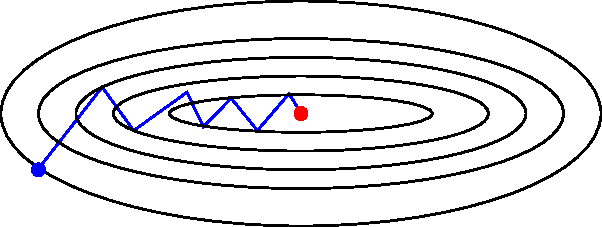
\includegraphics[width=.5\textwidth]{figures/optimization/optimization_batch_gd}
  \caption{Batch Gradient Descent: it needs to decrease the error on every
  step, if not, then the parameters are not right}
\end{figure}

\begin{figure}[h]
  \centering
  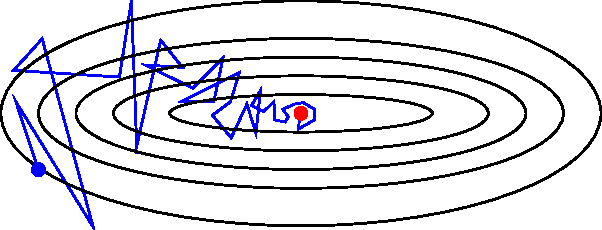
\includegraphics[width=.5\textwidth]{figures/optimization/optimization_stochastic_gd}
  \caption{Stochastic Gradient Descent: the error may increase ocasionally}
\end{figure}

\section{Summary of rates of convergence}

Given the problem parameters

\begin{itemize}
  \item $D$: diameter of the domain
  \item $B$ Lipschitz-constant
  \item $L$ smoothnesss constant
  \item $\mu$ strong convexity constant
\end{itemize}


\begin{table}[h]
  \def\arraystretch{1.4}
  \centering
  \begin{tabular}{|c|c|c|}
    \hline
    & \textbf{convex} & \textbf{strongly convex} \\
    \hline
    nonsmooth & deterministic: $BD/\sqrt{t}$ & deterministic: $B^2/(t\mu)$ \\
              & stochastic: $BD/\sqrt{n}$ & stochastic: $B^2/(n\mu)$ \\
    \hline
    smooth & deterministic: $LD^2/t^2$ & deterministic: $\exp(-t\sqrt{\mu/L})$ \\
           & stochastic: $LD^2/\sqrt{n}$ & stochastic: $L/(n\mu)$ \\
           & finite sum: $n/t$ & finite sum: $\exp(-t/(n+L/\mu))$ \\
    \hline
    quadratic & deterministic: $LD^2/t^2$ & deterministic: $\exp(-t\sqrt{\mu/L})$ \\
              & stochastic: $d/n + LD^2/n$ & stochastic: $d/n + LD^2/n$ \\
    \hline
  \end{tabular}
  \caption{Summary of rates of convergence}
\end{table}

\section{Conclusions}

\begin{itemize}
  \item Statistics with our without optimization
    \begin{itemize}
      \item Significance of mixing algorithms with analysis
      \item Benefits of mixing algorithms with analysis
    \end{itemize}
  \item Open problems
    \begin{itemize}
      \item Non-parametric stochastic approximation (Dieuleveut and Bach, 2014)
      \item Characterization of implicit regularization of online methods
      item Structured prediction
      \item Going beyond a single pass over the data (/testint performance)
      \item Parallel and distributed optimization
      \item Non-convex optimization (Reddi et al., 2016)
    \end{itemize}
\end{itemize}

\chapter{Supervised Learning and Text Classification by
\href{http://www.kyunghyuncho.me/}{Kyunghyun Cho}}

\section{Introduction to supervised learning with ANNs Wed.  11:30--13:00}

An overview on supervised learning, in which the input is described as a
validation set $D_{val}$ and a test set $D_{test}$

At the end we need to choose the hypothesis that best adjusts to our problem
between the availables. Examples of hyperparameters sets are in SVMs the
regularization parameters and the kernel, simiarly with Gaussian Processes with
the kernel and the parameters $\sigma^2$ and \emph{lenght-scale}.

In Artificial Neural Networks the hypothesis set is the set of architectures,
and hyperparameters. The architecture is commonly an directed acyclic graph
(DAG) with parameters, inputs, outputs and compute nodes (functions that are
often differentiable).

An example of architecture is a logistic regression where

\begin{equation}
  p_\theta(y=1|x) = \sigma(w^T x + b = \frac{1}{1 + \exp(-w^T x - b)}
\end{equation}

or a 3rd-order polynomial function.

The inference is done by forward propagation of the input to the output trhough
all the hidden layers.

Supervised learning tries to find a function $f_\theta(x)$, while in the case
of Neural Networks we can usually interpret it as computeing the conditional
probabilities guiven the input $p(y='|x)$. This is achieved by computing any
arbitrary output values from a network, then exponentiating every individual
prefdiction and dividing them by their sum (soft-max function).

The objective is that the training data is maximally maximized, by ensuring
that the maximum individual probabilities is maximized at the same time.

\begin{equation}
  \argmax_\theta \log p_\theta(D) = \argmax_\theta \sum_{n=1}^N \log
  p_\theta(y_n|x_n)
\end{equation}

We can also use the log-likelihood

\begin{equation}
  \text{Missing equation}
\end{equation}

\subsection{Loss minimization}

In order to minimize the loss it is necessaGraph Neural Networkry to use optimization techniques,
in the case of \glspl{ANN} is by using backpropagation to
compute the partial derivatives of the parameters with respect the input using
the chain rule of derivatives

\begin{equation}
  \frac{\partial(f o g)}{\partial x} = \frac{\partial f}{\partial
  g}\frac{\partial g}{\partial x}
\end{equation}

This differentiation is done automatically by
\href{https://github.com/HIPS/autograd}{autograd} which will implement the
Jacobian-vector product of each P node.

By doing backpropagation we obtain the gradient of the loss with respect to
every parameter $\theta$. Instead of computing the gradient for the full
dataset, it is common to use mini-batches with a method called Stochastic
Gradient Descent.

\begin{enumerate}
  \item Random subset of M training examples
  \item Compute the minibatch gradient
    \begin{equation}
      \Gradient L \sim 1/N' \sum_{n=1}^{N'} \text{missing part}
    \end{equation}
  \item Update the paraemters $\text{missing equation}$
  \item repeat until the validation loss stops improving
\end{enumerate}

However, this method will find a local minima in the training set, in order not
to overfit to the training data, a validation set is used to do an early stop.
This is one of the most important parts of the training as we want the minima
to be as near as possible to the dataset near.

\section{Text classification}

In text classificatio the input are sentences or paragraphs and the output is a
category to which the input belongs to (commonly a fixed number of $C$
categories).

Some of the particularities of using sentences as imputs is that they are of
variable size $X = (x_1, x_2, \dots , x_T)$ where every $x_t$ is a token from
a vocabulary $V$. This is done by automatically (or manually) splitting all the
individual words and creating an index of words that will form our vocabulary
$V$. Then every sentence is encoded by a sequence of integers. In this case we
are not tokenizing the words first by extracting any meaning of the word, in
this sense the words ``cat'' and ``cats'' have completly independent indices.

At the end the words are encoded as one-hot-encoding with a bit to 1 for the
corresponding index. This will be given to the \gls{ANN} and will be fordard
propagated to obtain a hidden representation $e_i$. This can be interpreted as
a table lookup from a word to a hidden embedding (eg. a fixed matrix $W$ of
  dimmension $\text{\#tokens} \times \text{\#arbitrary dimesion}$ that is
multiplied by the binary token).

The representation of a sentence is a continuos bag-of-words, this means that
we ignore the order of the words in the sentence, and average the corresponding
token vectors. The method has been proven to be very useful in the works
Iyyer2016, cho2017, and in FastText by Bojanowski2017.

\subsection{How to represent a sentence}

When the order of the words is important, it is possible to encode every set of
words. For example, Relation Network: skip bigrams consider all the possible
pairs of tokens and averages all the relationship vectors. The relations
between words can be encoded depending on the problem, we could consider that
the order of the bigrams is not important, only interested on bigrams of
contiguous words, all the possible pairs, or skip some words.

With the previous idea is possible to use Convolutional Neural Networks in
order to convolve the the ``look up table'' trough the input
\cite{kim2014convolutional}.

The CNN can also represent the bigram representations, and it is possible to
learn a weight vector that will choose how many words are important. Look at
the relation between Relational Networks and Convolutional Neural Networks.

\subsubsection{Self-attention 11:30--13:00}

Self-attention is a generalization of a CNN and RN that is able to capture
long-range dependecies with a single layer. It can also ignore irrelevant
long-term dependencies. Also mention generalization with multi-head and
multi-hop attention.

Using a Recurrent Neural Network we can create an online representation of a
sentence by reading every word and storing their representation in the
recursive hidden representation. This allows a cost of $O(T)$ instead of the
$O(T^2)$ necessary to do all the word pairs.

The representation that is generated by the RNN can encode the representation
of a region of the text given it's context. This can then be feeded to the
previously seen atention model that can learn the weighted sum of the context.

In ``Fully character-level neural machine translation without explicit
segmentation'' \cite{lee2016fully} the authors stack a RNN on top of CNNs.

\section{Natural Language Models}

\subsection{Autoregressive language modelling}

The autoregressive sequence modelling assumes that the past tokens influence
the current token as

\begin{equation}
  p(X) = p(x_1)p(x_2|x_1)\cdots p(x_T|x_1,\dots,x_{T-1})
\end{equation}

this holds true given the conditional distribution assumption.

With this method, an unsupervised method is transormed in $T$ smaller
supervised problems.

One think to keep in mind from a question that was asked is that altough the
marginalisation of $p(X)$ should sum to one, in real cases with RNNs this is
not always true. Possibly because of the parametrization.

The autoregressive sequence modelling can be represented as

\begin{equation}
  p(X) = \prod_{t=1}^T p(x_t|x_{<t})
\end{equation}

In order to score a sentence we can compare the output of the Autoregressive
model for several sentences and use softmax to obtain ``probabilities'' (values
between 0 and 1 that sum to one) for each sentence.

\subsection{N-Gram language models}

Before \glspl{ANN} were used, the idea about ussing the conditional probabilities was
already used on a smaller scale with N-gram models. In this case the $N$ needs
to be decided in advance.

\begin{align}
  p(x|x_{-N},x_{-N+1},\dots,x_{-1}) = \frac{p(x_{-N},x_{-N+1},\dots,x_{-1}, x)} {\sum_{x \in V}p(x_{-N},x_{-N+1},\dots,x_{-1}, x)}
\end{align}

The process then is to get the dataset and count the frequencies of every
occurrence of the tokens $\dots,x_{N-1}$ followed by all the possible tokens
$x$.

There are two main issues that araise by ussing frequentist N-Grams

\begin{enumerate}
  \item Data sparsity: lack of generalization
    \begin{itemize}
      \item If using a 3-gram model you find 3 words that never happened again,
        the product of probabilities will be zero independently on the rest.
      \item One possible solution is to use smoothing by adding a small
        constant
      \item Another solution is to try with all $n \in \{N,\dots,1\}$
    \end{itemize}
  \item Inability to capture long-term depenfdencies
\begin{itemize}
  \item By choosing a fixed $N$ we may lose long term dependencies.
\end{itemize}
\end{enumerate}

\subsection{Neural N-Gram Language Model}

\cite{bengio2003neural} solved some of the previous issues by using the
hidden representation of a Neural Network instead of the tokens. In the
continuous vector space the similar tokens or phrases are nearby.

Some other work on the same direction is \cite{mikolov2013distributed},
, \cite{pennington2014glove}, \cite{le2014distributed}.

An example of this application is the generalization of sentences that never
happened by realizing that some words share some similarities (eg. numbers). An
example was shown in which sentences with the 2-grams ``three teams'', ``four
teams'' and ``four groups'' are able to generalise to the bigram ``three
groups'' by realizing that three and four share a similar continuous space, and
that before groups there could be a number.

In practice

\begin{enumerate}
  \item Collect TODO missing steps
\end{enumerate}

\subsection{Convolutional Language Models}

Convolutional Neural Networks allow to extend the context size by applying the
convolution through larger parts of the text (see kalchbrenner et al, 2015 and
Dauphin et al 2016, ByteNet by \cite{kalchbrenner2016neural}, PixelCNN,
WaveNet, \dots)

Gated convolutional language model by Dauphin 2016 \cite{dauphin2016language}


\subsection{CBoW Language Models (infinite context)}

The idea is similar to the LM of using averages instead of concatenation.

\subsection{Recurrent Language Models}

An RNN can summarize all the tokens seen until $x$ into a continuous vector
representation Mikolov et al, 2010 \cite{mikolov2010recurrent}.

\subsection{Recurrent Memory Networks}

The work of Tran et al., 2016 \cite{tran2016recurrent} combines RNNs to compress the context into a
continuous vector representation with the attention model that learns the
weighting of the context.

\section{Recurrent Networks and Backpropagation}

Consider the full path from a parameter $\theta$ to the loss $l$. The
backpropagation consists on computing the gradient of the $l$ with respect to
the previous node and multiply by the Jacobian matrix of every step back to the
parameter $\theta$.

\begin{equation}
  \Jac_{h^{t+1}}^{h^t} = W^T \text{diag}(\tanh'(a^t))
\end{equation}

Because the Jaciobians are multiplied by every backpropagation step, this means
that

\begin{itemize}
  \item If $W > 1$ (the upperbound of ) the norm blows up, exploding gradient
  \item If $W < 1$ (the upperbound of) the norm shrinks to zero, vanishing
    gradient
\end{itemize}

\begin{equation}
  || \prod_{t'=t}^{} || \le  || \Jac || \text{TODO missing part}
\end{equation}

\subsection{Gated recurrent units}

These type of networks allow to skip some of the paths in order to avoid the
exploding or vanishing gradient.

\begin{itemize}
  \item Adaptive shortcut:
  \item Candidate update + pruning
  \item Update gate: $u_t = \sigma(W_uh_{t-1} + U \cdots$
  \item reset gate $r_t = \sigma(W_rh_{t-1} + U_rx + b_r)$
\end{itemize}

\subsection{Lessons from GRU/LSTM}

\begin{itemize}
  \item Credit assignment over a long path of computation is difficult
    \item Adaptive shorcut or skip-connection helps avoid credit dilution
      \item Gates are an effective way to focus credit assignment
\end{itemize}

\section{Neural Machine Translation 14:30--16:00}

\subsection{History of machine translation}

The original idea was to get a text from one language, (1) perform a
morphological analysis, (2) a syntactic analysis, (3) semantic analsysis, (4) a
semantic composition and obtein an interlingua text that can be transformed
back to any other language Borr, Hovy and Levin 2006 \textbf{TODO missing
citation}.

Allen 1987 ieee icnn, a brief resurrection of Neural Networks in 1997 by
Castano and Casacuberta 1997 \cite{castano1997machine}, then in 2006 Schwenk
2006 \cite{schwenk2006continuous} as a filter source to SMT to \gls{ANN} to target sentence, then Devlin 2014 from
source to SMT + \gls{ANN} to target sentence, then source to
\gls{ANN} to target sentence.

\subsection{Encoding: Token representation}

First it is necessary to build a source and target vocabulary of unique tokens
(for each language). Then transform the text into the set of tokens. Then
encode the token sentences into sentence representation vectors, being careful
not to compress the sentences into small vectors that may lose useful
information.


\subsection{Decoding: conditional language modeling}

Using autoregressive networks we are interested in predicting the posterior
probability

\begin{equation}
  p(Y|X) = \prod_{t=1}^T p(y_t|y_{t-1}, X)
\end{equation}

Look at the RNN Neural Machine Translation by Bahdanau et al., 2015
\cite{bahdanau2014neural}. The model uses the target sentence (and what has
been translated until the current moment) in order to generate the following
prediction.

\begin{enumerate}
  \item Encode: read the entire source sentence to know what to translate
  \item Attention:
  \item Decode:
  \item Repeat 2 to 3 until the end-of-sentence (token) is achieved
\end{enumerate}

This method achieved performance as good as the current state-of-the-art
alternative at the moment phrase-based machine translation (PBMT).

At translation time every predicted word of the sentence had an associated
vector of weights that indicted the source words involved, altough the model
was trained only with pairs of text without any extra supervision. We should
consider that every token of the source sentence is at the same time associated
with a context in its language (see \cite{jean2015montreal}).

\subsection{In practice}

Available frameworks

\begin{itemize}
  \item Nematus \cite{sennrich2017nematus}
  \item OpenNMT-py \cite{opennmt}
  \item FairSeq \cite{gehring2017convs2s}
  \item Sockeye \cite{Sockeye:17}
\end{itemize}

\section{Current and ongoing projects}

Multilingual translation, real-time translation, and character level
translation.

\subsection{Multilingual translation}

A common approach has been to use a pivot language to translate languages
without lots of examples. For example, translate korean to Japanese and then to
English as the corpus between them is larger than the Korean to English.

With this idea, there has been some work to generate a pivot common language
that is automatically learned in an \gls{ANN}. For example, an encoder/decoder
aproach in \cite{firat2016multi, firat2016zero} creates one encoder per source
and decoder per target, and a model is learned for every pair. Later Johnson et
al, 2016, Ha et al, 2016, Lee et al 2017, and Gu et al, 2018 work on an
Universal \dots

A current limitation is these methods drastically depend on the different
amount of available data in each language. The models start ignoring the less
frequent language. However, if given the same proportions of samples for every
language they may overfit to the less frequent one because of the multiple epochs
run on one language compared to the other.

Some work to solve this problem is being done with Meta-Learning MAML in
\cite{finn2017model}. The difference with multitask learning is that  \dots

Another idea is to create the unsupervised lookup tables to convert word tokens
into continuous vectors ussing big corpus of different languages. In this
manner, words with simmilar meanings will fall into similar regions (see
\cite{artetxe2017unsupervised}). In this case, the overfiting is less probable
to happen as the lookup table is only learning a mapping of tokens to a
continuoius space, but not the translation. Then, the translation model is
trained on top of it.

\subsection{Real-Time Translation (learning to decode)}

learning to translate in real-time with neural machine translation
\cite{gu2016learning}

In order to generate the best translation it is possible to generate several
and then select the most probable one. However, ocasionally it may happen that
after several words are translated the topic changes and the best translation
may be a different one. In order to solve this the Beam Search keeps track of
parallel best translations and is able to switch to another one at any point if
necessary.

\begin{mybox}
\textbf{Exploiting the hidden activation}

In a Deep Neural Network huge information in the hidden layers is usually
discarded in order to predict a class; obtaining at the end a binary
prediction. However, the hidden information has rich information about the
original input that can be exploited.
\end{mybox}

By using the hidden information the performance of several methods was
increased \cite{gu2016learning}.

\chapter{Causality by \href{https://staff.fnwi.uva.nl/j.m.mooij/}{Joris Mooij}}

There are many questions in science that are casual (eg. climatology,
healthcare, \dots).

\section{Introduction}


Causation is not correlation (gives example with chocolate consumption being
correlated with number of nobel prizes in different countries, while there is
no actual correlation between both).

In order to represent causal relations we can use \emph{causal graphs}
(directed graphs) in wich nodes are variables $X_n$ from (a vocabulary?) $V$.
While directed edges indicate that the first variable causes direclty another
variable respect to $V$. An example of a cyclic graph where every adjacent
variable is directly connected to its neighbours is the encoding of standing
domino pieces.

It is possible to modify the \emph{causal graph} with an \emph{intervention},
in the example the domino piece $X_2$ is glued to the floor, removing the
direct connections from other pieces to $X_2$, but possibly keeping a
connection from $X_2$ to the adjacent (in case an external user can still force
$X_2$ to fall).

A \emph{perfect (``surgical'', ``atomic'') intervention} on a set of variables
$X \subseteq V$, is an external enforced change of the system (eg. the
previous example).

A \emph{confounder} is a latent common cause:

\begin{mybox}
  $H$ is a confounder of $X$ and $Y$ if:
  \begin{enumerate}
    \item $H$ causes $X$ directly w.r.t. $\{X, Y, H\}$
    \item $H$ causes $Y$ directly w.r.t. $\{X, Y, H\}$
  \end{enumerate}
\end{mybox}

We will denote latent confounders by \emph{bidirected edges} in a causal graph.

\section{Defining causality in terms of probabilities}

\emph{Simpson's paradox} shows that if we interpret the probabilities as causes
we may make wrong decisions. As an example, shows the recovery rate of a drug
test in which depending on the groups separation the most probable outcome
changes.

\begin{mybox}
\begin{enumerate}
  \item The probability of recovery is higher for patients that took the drug
    \begin{align}
      p(\text{recovery}|\text{drug}) > p(\text{recovery}|\text{no drug})
    \end{align}
  \item For both male and female patients the relation was oposite
    \begin{align}
      p(\text{recovery}|\text{drug, male}) <& p(\text{recovery}|\text{no drug,
      male}) \\
      p(\text{recovery}|\text{drug, female}) <& p(\text{recovery}|\text{no drug,
      female})
    \end{align}
\end{enumerate}
\end{mybox}

\emph{endogenous variables} are binary variables that we are interested in.

\emph{Exogenous variables} are latent, independent binary variables that affect
externally the state of our endogeneous variables.

A \emph{Structureal Causal Model (SCM)}, also knwon as \emph{Structural
Equation Model (SEM)}, is a tuple \dots

There is one Structural equations  per endogenous variable.

\begin{enumerate}
  \item a product of standard measures \dots
  \item a product of standard measures \dots
  \item Measurable mapping \dots
  \item A product probbility measure\dots
\end{enumerate}

An augmented functional graph $G^a(M)$ depicts the exogenous variables while
the functional graph $G(M)$ doesn't.

\begin{mybox}
  If $M$ has no \emph{self-loops}, the causal graph of $M$ is a subgraph of the
  functional graph $G(M)$.
\end{mybox}

\begin{definition}
We call the family of sets of probability distributions of the solutions of
$M_{do(l,E_l)}$ \dots
\end{definition}

some of the previous points are teh basic difference between causal models and
probabilistic models.

We donote a marginalization of the model $M$ with respect two variables $X_2$
and $X_4$ as $M^{\backslash\{2,4\}}$.

See the following extra references \cite{de2013global}, and
\cite{bongers2018random}, \cite{blom2018generalized},
Bongers et al., 2018.


\begin{definition}
  Definitions of: Independence and conditional independence
\end{definition}

\begin{definition}
  Definition of: nodes blocking a path
\end{definition}

\begin{theorem}
  For an \emph{acyclic} SCM, \dots
\end{theorem}

\emph{Reichenbach's} principle of common cause, the dependence $X | Y$

The Reichenbach's Principe may fail in case of \emph{selection bias} (related
with the explaining away problem)


\section{Causal Inference: Predicting Causal Effects}

\begin{theorem}
  Back-Door Criterion \cite{pearl2000causal}
\end{theorem}

\section{Resolving Simpson's paradox}

It is important to realize that ``seing'' is not the same as ``doing''.

\begin{itemize}
  \item $p(R = 1|D = 1)$: the probability that somebody recovers, given the
    observation that the person took the drug.
  \item $p(R = 1| \text{do}(D=1))$: the probability that somebody recovers, if
    we force the person to take the drug.
\end{itemize}

In practice randomized control trial

\begin{mybox}
  A \textbf{randomized controlled trial} (or randomized control trial;[2] RCT) is a type
of scientific (often medical) experiment which aims to reduce bias when testing
a new treatment. The people participating in the trial are randomly allocated
to either the group receiving the treatment under investigation or to a group
receiving standard treatment (or placebo treatment) as the control.
Randomization minimises selection bias and the different comparison groups
allow the researchers to determine any effects of the treatment when compared
with the no treatment (control) group, while other variables are kept constant.
The RCT is often considered the gold standard for a clinical trial. RCTs are
often used to test the efficacy or effectiveness of various types of medical
intervention and may provide information about adverse effects, such as drug
reactions. Random assignment of intervention is done after subjects have been
assessed for eligibility and recruited, but before the intervention to be
studied begins. -- \textbf{Wikipedia}
\end{mybox}

\section{Causal Discovery: from data to causal graph}

Randomized controlled trials \cite{fisher1935design} are one solution to avoid
previously seen problems.

\begin{enumerate}
  \item Divide patients into two groups: treatment and control randomly
  \item Patients with the treatment group are forced to take a drug, and
    patients in the group are forced to not take the drug (but to take a
    placebo instead): $D = C$
  \item Estimating the causal effect of the drug now becomes a standard \dots
  \item \dots
\end{enumerate}

\subsection{Local Causal Discovery (LCD)}

Simple method that Joris Mooij likes

\section{Practical aplication}

It is possible to apply $k$-fold Cross-validation to the observational data and
interventional data in order to estimate the test performance.

\section{Conclusions}

Additional readings: Causality: Models reasoning and inference, pearl 2000.
Constraint-based causal discovery for non-linear

\begin{itemize}
  \item Elements of causal inference, foundations and learning algorithms by
    Peters, Janzing, Scholkopf 2017 %\cite{peters2017elements}
  \item Causation, prediction and search by spirtes, glymour, scheines 2000
    %\cite{spirtes2000causation}
  \item correlation and causation by Wrights 1921
  \item Causal inference in statistics: an overview by Pearl 2009
  \item Simpson's paradox: an anatomy by Pearl 1999 %\cite{pearl1999simpson}
  \item Causality: models, reasoning and inference by Pearl 2000
    %\cite{pearl2003causality}
  \item Theoretical aspects of cyclic structural causal models by
    Bongers, Peters, Scholkopf, Mooij 2018 %\cite{bongers1611theoretical}
  \item Markov properties for graphical models with cycles and latent
    variables by Forré, and Mooij 2017 %\cite{forre2017markov}
\end{itemize}

Some possible aplications of Causal inference could be:

\begin{itemize}
  \item Transfer learning
  \item Domain adaptation
  \item Reinforcement learning
\end{itemize}

What tools or framewors: \textbf{there are no tools yet}, R package for
individual methods. Literature and the implementations are scattered,
\textbf{necessary to unify!}.

\chapter{Reinforcement Learning by \href{http://www.jan-peters.net/}{Jan Peters}}

Fri. 14:30--16:00

\section{Optimal Control Systems}

Data to model to value function to policy back then to data.

\subsection{Markov Decision Problems}

A stationary MDP is defined as

\begin{itemize}
  \item a state space $s \in S$
  \item action space $a \in A$
  \item transition dynamics $P(s_{t+1}| s_t, a_t)$
  \item reward function $r(s,a)$
  \item initial state probabilities $\mu_0(s)$
\end{itemize}

The Markov property says that the transition dynamics depends only on the
current time step.

\begin{equation}
  P(s_{t+1}|s_t, a_t, s_{t-1}, a_{t-1}, \dots) = P(s_{t+1}|s_t, a_t)
\end{equation}


\subsection{Basic reinforcement learning loop}

The objective is to maximize the expected long-term reward

\begin{equation}
  J_\theta = \Expected_{\mu_0, P, \pi} [\sum_{t=1}^{T-1}\gamma^t r(s_t, a_t)]
\end{equation}

The algorithmic description of the value iteration

\begin{itemize}
  \item Init: $V_T^*(s) \leftarrow r_T(s), t=T$
    \begin{itemize}
      \item Compute Q-Function for time step t (for each state action pair)
        \begin{equation}
          Q_t^*(s,a) = r_t(s,a) + \gamma \sum_{s'} P_t (s'|s,a)V_{t+1}^*(s')
        \end{equation}
      \item Compute V-Function for time step t(for each state) (TODO, check if
        next equation is max or argmax)
        \begin{equation}
          V_t^*(s) = \max_a Q_t^*(s,a)
        \end{equation}
    \end{itemize}
  \item Repeat: $t=t-1$
  \item Until $t=1$
  \item REturn: Optimal policy for each time step
    \begin{equation}
      \pi_t^*(s) = \argmax_a Q_t^*(s,a)
    \end{equation}
\end{itemize}

The Bellman Equation (Bellman Principle of Optimality)

\begin{equation}
  V^*(s) = \max_a (r(s,a) + \gamma \Expected_p[V^*(s')|s,a)
\end{equation}


See Policy evaluation with temporal differences: a survey and comparison
\cite{dann2014policy}

When the max is expensive is possible to use the \emph{Policy Iteration}
method:

\begin{enumerate}
  \item Policy evaluation: Estimate quality of states (and actions) with
    current policy
  \item Policy improvement: Improve policy by taking actions with the highest
    quality
\end{enumerate}

\subsection{Linear Quadratic Gaussian Systems}

A Linear Quadratic Regulator (LQR) system is defined as

\begin{itemize}
  \item state space $x in \Real^n$
  \item action space $u in \Real^m$
  \item linear transition dynamics with Gaussian noise
    \begin{equation}
      p_t(x_{t+1}|x_t, u_t) = \Normal(x_{t+1}|A_t x_t + B_t u_t + b_t, \Sigma_t)
    \end{equation}
  \item quadratic reward function
    \begin{align}
      r_t(x,u) =& (x-r_t)^T R_t(x-r_t) + u_t^T H_t u_t \\
      r_t(x) =& (x-r_T)^T R_T(x-r_T)
    \end{align}
  \item initial state density
    \begin{equation}
      \mu_0(x) \Normal(x|\mu_0, \Sigma_0)
    \end{equation}
\end{itemize}

See Stefan Schaal, Christopher G. Atkeston 1998 \cite{schaal1998constructive}

The LQR systems need the initial point to be linearly related to the optimal
point (eg. keeping a stick balanced upwards). However, they can not solve
situations in which it is necessary a non-linear component (eg. if the stick
  starts from a hanging position, and it needs some sinuidal movement before it
can reach the upward position).

See work by Emo Todorov and Yuval Tassa on Incremental LQG (a simplification of
  Differential Dynamic Programming by Dyer and McReynolds 1969
\cite{dyer1969optimization})

With Optimal control we can compute optimal policies but only on

\begin{enumerate}
  \item Discrete Systems: (but world is not discrete)
  \item Linear Systems, Quadratic Reward, Gaussian Noise (LQR): (but the world
    is not linear)
  \item Along an optimal trajectory: (it is really hard to find)
\end{enumerate}

For these reasons we need to approximate.

\section{Value Function Methods}

Data to value function to policy to data.

One of the principles is that ``all models are wrong, but some are useful''. In
the previous section we created perfect models, but they may not be match the
real world. In that case, there can be drastical problems.

The \emph{Classical Reinforcement Learning} postulate is to solve the optimal
control problem by learning the value function and not the model.

\subsection{Markov Decision Processes (MDP)}

Infinite Horizon with a discounted reward parameter $\gamma$

Updates the value function based on samples $D = \{s_i, a_i, r_i, s_i'\}$

\subsection{Temporal difference learning}

We are incorporating an error value into the prediction of the states (see
  Reinforcement learning, rich sutton and andy barto, 1998
  \cite{sutton1998reinforcement}.

Withe our estimate we can compute the TD error and make a decision

\begin{itemize}
  \item if the estimation was higher, we decrease the prediction
  \item if the estimation was lower, we increase the prediction
\end{itemize}

\begin{enumerate}
  \item Init $V_0^*(s) \leftarrow 0$
  \item Repeat $t=t+1$
    \begin{itemize}
      \item Observe transition $(s_t,a_t,r_t,s_{t+1})$
      \item Compute TD error $\delta_t = r_t + \gamma V_t(s_{t+1}) - V_t(s_t)$
      \item Update V-Function $V_{t+1}(s_t) = V_t(s_t) + \alpha\delta_t$
    \end{itemize}
  \item until convergence of $V$
\end{enumerate}

But we do not want deterministic policies as these will not explore the space,
for that reason there are at least two policy for exploration

\begin{enumerate}
  \item Epsilon-Greedy Policy
  \item Soft-Max Policy (it has an important temperature parameter $\beta$)
\end{enumerate}

Update equations for learning the Q-function $Q(s,a)$

\begin{equation}
  Q_{t+1}(s_t,a_t) =  \dots
\end{equation}

In wich it is necessary to estimate the future action $a_?$. There are two
methods

\begin{enumerate}
  \item Q-learning: $a_? = \argmax_a Q_t(s_{t+1}, a)$
  \item SARSA: $a_? = a_{t+1}$, where $a_{t+1} \from \pi(a|s_{t+1})$
\end{enumerate}

\subsection{Approximating the value function}

Instead of creating the matrix $V$ we can approximate with any function
approximation method (see Dann et al: Policy evaluation with temporal
differences: a survey and comparison, JMLR, 2014 \cite{dann2014policy}).

Some remarks on temporal difference learning

\begin{itemize}
  \item It si not a proper stochastic gradient descent
  \item As the target values $V^\pi(s)$ change after each parameter update
  \item This ``ignoreance'' introduces a bias in our optimization
  \item \dots
\end{itemize}

\subsection{Batch-Mode Reinforcement Learning}

Online methods are typically data-inefficient as they use only once every
sample. The rehuse of the samples has been done in Least-squares temporal
difference learning and fitted q-iteration (Tree-Based batch mode reinforcement
learning \cite{ernst2005tree}, Batch reinforcement learning
\cite{lange2012batch}).

In Q-iteration we do as in Value-iteration, but we use Supervised Learning
methods to approximate the ? function.

See Reinforcement learning in robot soccer, 2009
\cite{riedmiller2009reinforcement}.


\section{Policy Search}

From data to policy and back to data.

see Reinforcement learning of motor skills with policy gradients, 2008
\cite{peters2008reinforcement}.

\subsection{Black-box approaches}


\begin{itemize}
  \item Perturb the parameters of your policy: $\delta J = J(\theta + \delta
    \theta) - J(\theta)$
  \item Approximate J by the first order Taylor approximation $J(\theta +
    \delta\theta) = J(\theta) + \frac{\partial
    J(\theta)}{\partial\theta}\delta\theta$
  \item Solve for $\frac{\partial J(\theta)}{\partial \theta}$ in a least
    squares sense (linear regresssion).
\end{itemize}

See a large classs of algorithms includes: Kiefer-Wolfowitch procedure,
Robbins-Monroe, Simultaneous Perturbation Stochastic Approximation SPSA,\dots

\subsection{Likelihood-Ratio Policy Gradient methods}

The expected long term reward $J(\theta)$ can be weritten as expectation over
the trajectory distribution.

\section{Key problems}

\begin{enumerate}
  \item no notion of data in the generic problem formulation
  \item optimization bias problematic with data
  \item role of tfeatures is unclear in most methods
\end{enumerate}
\bibliographystyle{apalike}
\bibliography{references}

\include{chapters/chap9}
\chapter{Probabilistic Numerics: Nano-machine-learning by
\href{http://www.robots.ox.ac.uk/\~mosb/}{Michael A Osborne}}

9:30--11:00

Numerics is becoming one of the important fields of Machine Learning.

\begin{mybox}
  In numerical analysis, numerical integration constitutes a broad family of
  algorithms for calculating the numerical value of a definite integral, and by
  extension, the term is also sometimes used to describe the numerical solution
  of differential equations. This article focuses on calculation of definite
  integrals. The term numerical quadrature (often abbreviated to quadrature) is
  more or less a synonym for numerical integration, especially as applied to
  one-dimensional integrals. Some authors refer to numerical integration over
  more than one dimension as cubature;[1] others take quadrature to include
  higher-dimensional integration. -- Wikipedia
\end{mybox}

The answer to a numeric problem can only be approximated, e.g.

\begin{equation}
  F = \int_{-3}^3 f(x) dx
\end{equation}

for

\begin{equation}
  f(x) = \exp(-(\sin(3x))^2 - x^2)
\end{equation}

This can be as long as 30 polinomic elements. Altough we can not use it
analytically, we can get an approximated answer with a computer.

A motivation:

\begin{enumerate}
  \item numeric \emph{error} is significant
  \item numeric methods are generic
  \item our numerics problems tax our computation
\end{enumerate}

Some important parts of the integration to have in mind:

\begin{itemize}
  \item The data: are the evaluations, or
  \item Predictand: is the integral
  \item Decisions: \dots
\end{itemize}

Bayesian quadrature is probabilistic numerics for intergration

\begin{mybox}
  Bayesian Quadrature is a statistical approach to the numerical problem of
  computing integrals and falls under the field of probabilistic numerics. It
  can provide a full handling of the uncertainty over the solution of the
  integral expressed as a Gaussian Process posterior variance. It is also known
  to provide very fast convergence rates which can be up to exponential in the
  number of quadrature points n.[5] --
  \href{https://en.wikipedia.org/wiki/Numerical_integration}{Wikipedia}
\end{mybox}

With a \emph{Gaussian process} prior for the integrand, the \emph{integral is
joint Gaussian.}


\begin{figure}[h]
\centering
\pgfplotsset{
colormap={whitered}{color(0cm)=(white); color(1cm)=(orange!75!red)}
}

\begin{tikzpicture}[
    declare function={mu1=1;},
    declare function={mu2=2;},
    declare function={sigma1=0.5;},
    declare function={sigma2=1;},
    declare function={normal(\m,\s)=1/(2*\s*sqrt(pi))*exp(-(x-\m)^2/(2*\s^2));},
    declare function={bivar(\ma,\sa,\mb,\sb)=
        1/(2*pi*\sa*\sb) * exp(-((x-\ma)^2/\sa^2 + (y-\mb)^2/\sb^2))/2;}]
\begin{axis}[
    colormap name=whitered,
    width=.8\linewidth,
    view={45}{65},
    enlargelimits=false,
    grid=major,
    domain=-1:4,
    y domain=-1:4,
    samples=15,
    xlabel=$x$,
    ylabel=$\int f(x) xd$,
    zlabel={$P$},
    colorbar,
    colorbar style={
        at={(1,0)},
        anchor=south west,
        height=0.25*\pgfkeysvalueof{/pgfplots/parent axis height},
        title={$\int f(x) xd$}
    }
]
\addplot3 [surf] {bivar(mu1,sigma1,mu2,sigma2)};
\addplot3 [domain=-1:4,samples=31, samples y=0, thick, smooth] (x,4,{normal(mu1,sigma1)});
\addplot3 [domain=-1:4,samples=31, samples y=0, thick, smooth] (-1,x,{normal(mu2,sigma2)});

\draw [black!50] (axis cs:-1,0,0) -- (axis cs:4,0,0);
\draw [black!50] (axis cs:0,-1,0) -- (axis cs:0,4,0);

\node at (axis cs:-1,1,0.18) [pin=165:$P(x_1)$] {};
\node at (axis cs:1.5,4,0.32) [pin=-15:$P(x_2)$] {};
\end{axis}
\end{tikzpicture}
\end{figure}


Monte Carlo is also Bayesian quadrature

The motnte caro estimate is

\begin{equation}
  \int f(x) p(x) dx \backsimeq 1/N \sum_{i=1}^N f(x_i)
\end{equation}

is a maximum a-posteriori under the (imporoper) prior

\begin{equation}
  p(f) = \lim_{e \ra 0} GP(0, \theta^2 \Indicator(x = x') + c^{-1})
\end{equation}

TODO missing conclusion for last equation

Managing parameters $\theta$ requires the model \dots

\begin{equation}
  \int f(x|\theta) d\theta \text{  missing equation}
\end{equation}


In optimization it is not enought looking for the higher likelihood value, but
we are looking for the highest mass. This is picks with larga areas around.

\begin{equation}
  p(data) \backsimeq  \text{  missing}
\end{equation}

We prefer \emph{flat optima} to \emph{pick optima} preciselly because of the
mass.

In Monte Carlo estimator

\begin{equation}
  \int f(x) p(x) dx \backsimeq 1/N \sum_{i=1}^N f(x_i)
\end{equation}

ignores relevant information and assumes certain sample distribution (see Monte
  Carlo is Fundamentally unsound \cite{o1987monte})

\emph{Warped sequential active Bayesian integration (WSABI)} uses a loss that
is the uncertainty in the integrand (see Sampling for inference in
Probaiblistic models with fast bayesian quadrature, NIPS
\cite{gunter2014sampling})

\begin{mybox}
  We propose a novel sampling framework for inference in probabilistic models: an
active learning approach that converges more quickly (in wall-clock time) than
Markov chain Monte Carlo (MCMC) benchmarks. The central challenge in probabilistic
inference is numerical integration, to average over ensembles of models or
unknown (hyper-)parameters (for example to compute the marginal likelihood or
a partition function). MCMC has provided approaches to numerical integration that
deliver state-of-the-art inference, but can suffer from sample inefficiency and poor
convergence diagnostics. Bayesian quadrature techniques offer a model-based
solution to such problems, but their uptake has been hindered by prohibitive computation
costs. We introduce a warped model for probabilistic integrands (likelihoods)
that are known to be non-negative, permitting a cheap active learning
scheme to optimally select sample locations. Our algorithm is demonstrated to
offer faster convergence (in seconds) relative to simple Monte Carlo and annealed
importance sampling on both synthetic and real-world examples. -- Abstract from
\cite{gunter2014sampling}
\end{mybox}

In global optimization

\begin{itemize}
  \item Data: evaluation
  \item Predictand: minimizer
  \item Decisions: location
\end{itemize}

Bayesian optimisation is probabilistic numerics for global optimization

The loss for optimisation could be

\begin{enumerate}
  \item the lowwest evaluation (value): Some times it is really important to
    choose the best option, but not care about the uncertainty
  \item the uncertainty in the minimiser (location-information): e.g. if you
    create the model in synthetic data, it is important to evaluate the
    uncertainty on the new real data
  \item the uncertainty in the minimum (value-information):
\end{enumerate}


\begin{itemize}
    \item
    \begin{equation}
      \lambda_{VL} = y_N
    \end{equation}
    \item
    \begin{equation}
      \lambda_{LIL} = \mathbb{\mathop{M}} (x_* | x_N, y_N, D_N)
    \end{equation}
\end{itemize}

Solving the intrinsic ``myopia'' of bayesian optimization methods (see GLASSES:
relieving the myopia of bayesian optimization \cite{gonzalez2016glasses})


\section{Upper confidence bound}

is the myopic acquisition function


\begin{equation}
  \text{missing equation}
\end{equation}

given a surrogate with mean $m(x_n)$ and variance $V(x_n)$


\section{Information-theoretic methods}

give alternative myopic implementations of va-ue.-information and
location-information losses:

% \begin{align}
%   \alpha_{LiL} = \Expected_{y_n} \mathbb{\mathop{H}}(x_*|y_n, x_n, D_n)
% \end{align}

these methods tend to be more exploratory

\section{Technology at work: The future of automation Tue. 9:30--11:00}


What are humans still good for?
\bibliographystyle{apalike}
\bibliography{references}

\chapter{Kernel methods by \href{http://www.gatsby.ucl.ac.uk/~gretton/}{Arthur Gretton}}

 Tue. 11:30--13:00

\begin{itemize}
  \item Testing goodnes of fit: Given a model $P$ and samples $Q$
  \item Dependence testing
\end{itemize}

Maximum mean discrepancy (MMD)

\section{Reproducing Hilbert spaces}

Definition (Inner product)

Let $H$ be a vector space over $\Real$. A function $k(x,x')$ is an inner
product of $x$.

\begin{theorem}
  Sums of kernels are kernels: Given $\alpha > 0$ and $k, k_1$ and $k_2$ all
  kernels on $\chi$, then $\alpha k$ and \dots are kernels.
\end{theorem}

\begin{theorem}
  Products of kernels are kernels:
\end{theorem}

\begin{theorem}
  Polynomial kernels:
\end{theorem}

A famous infinite feature space kernel, the exponentiated quadratic kernel

\begin{equation}
  k(x, x') = \exp\left(-\frac{||x-x'||^2}{2\sigma^2}\right)
\end{equation}

Smoothness in RKHS with exponentiated quadratic kernel

\begin{equation}
  f(x) = \sum_{i=1}^m \alpha_i k(x_i, x) = \sum_{t=1}^\infty f_l [\sqrt{\lambda_l}e_l(x)]
\end{equation}

\section{Interlude: divergence measures}

Integral probability metrics (substraction): wasserstein, MMD, TV

\begin{equation}
  D_H(P,Q) = \text{sup}_{g \in H} | E_{X \from P}g(X) - E_{Y \from Q}g(Y)|
\end{equation}

F-divergences: Pearson chi2, Hellinger, KL, TV

\begin{equation}
  D_f(P,Q) = \int_\chi q(x) f(\frac{p(x)}{q(x)})dx
\end{equation}

Notice the intersection TV (see \dots)

\section{Two-sample testing with MMD}


\begin{itemize}
  \item Null hypothesis: $H_0$ when $P = Q$ \\
    should see $\hat{MMD}^2$ close to zero
  \item Alternative hypotesis $H_1$ when $P \ne Q$ \\
    should see $\hat{MMD}^2$ far from zero
\end{itemize}

Set the treshold by shuffling the data from both classes and dividing into two
sets $P$ and $Q$. Then computing the $\hat{MMD}^2$ of $P$ and $Q$.

\section{Training GANs with MMD Wed. 9:30--11:00}

Generative Adversarial Networks are composed of a student (generator) and a
teacher (discriminator). The student is learning to generate samples and the
teacher is assesing if the generated samples are good or not. However, the
student could memorize one sample and improve this one until the teacher
asseses that it is always correct.

To improve the critic witness it is possible to add convolutional features to
be discriminated, and the teacher (critic) also needs to be trained (see MMD
GAN Li et al, NIPS 2017 \cite{li2017mmd}, Coulomb GAN Unterthiner et al., ICLR
2018 \cite{unterthiner2017coulomb})

Another idea is WGAN-GP (see Wasserstein GAN by Arjovsky et al. ICML 2017
\cite{arjovsky2017wasserstein}, WGAN-GP Gukrajani et al. NIPS 2017
\cite{DBLP:journals/corr/GulrajaniAADC17}).

New MMD GAN witness regulariser  (Arbel, Sutherland, Binkowski, G NIPS 2018),
based on semi-supervised learning regulariser by Bousquet et al NIPS 2004.

\subsection{The kernel inception distance (KID)}

The kernel inception distance 8by Binkowski, sutherland, arbel G ICLR 2018)
measures the similarity of the samples' representations in the inception
architecture (pool3 layer) MMD with kernel

\begin{equation}
  k(x,y) = (\frac{1}{d}x^Ty+1)^3
\end{equation}

Checks match for feature means, variances and skewness. It is unbiased?.

\section{Testing statistical dependence}

Example with captions of images of cats and dogs. First we obtain a good kernel
to compare images $k(x, x')$, and a good kernel to compare text $l(x, x')$.

\begin{itemize}
  \item Given: samples from a distribution $P_{XY}$
  \item Goal: are $X$ and $Y$ independent?
    \begin{equation}
      MMD^2(\hat{P}_{XY}, \hat{P}_X, \hat{P}_Y, H_k) =
      \frac{1}{n^2}\text{trace}(KL)
    \end{equation}
\end{itemize}

\subsection{Finding covariance with smooth transformations}

Illustration with a variable $X$ and $Y$ with a shape of a circle perimeter
with some gaussian noise. In this case the correlation between variables is 0,
but with certain witness functions for $w_x(X)$ and $w_y(Y)$ we can find a
correlation between them.

\subsection{Application: dependence detection across languages}

\begin{itemize}
  \item Testing task: detect dependence between English and French text
  \item k-spectrum kernel, $k=10$
\end{itemize}

\chapter{An introduction to Bayesian nonparametrics by
\href{http://sinead.github.io/}{Sinead Williamson}}

\section{The Dirichlet process}

\subsection{An urn representation}

\begin{itemize}
  \item Conditioned on $\phi$ \dots
\end{itemize}

\begin{align}
  p(z_i = k| z_{i:i-1} =& \int p(z_i = k| \pi) p(\pi|z_{1:i-1} d\pi \\
      =& \frac{\sum_{j=1}{i-1} \Indicator(z_j = k) + \alpha_k}{i - 1 + \sum_k
      \alpha_k}
\end{align}

\subsection{Exchangeability}

\begin{itemize}
  \item Changing the order of the observation does not change the probabilities:
    $p(r,g,g,r,b,r) = p(r,r,r,g,g,b)$
  \item This allows us to threat every data point as if it were the las one
    that we piked out
\end{itemize}

\subsection{Choosing the number of clusters}

\begin{itemize}
  \item The Dirichlet distribution is a great choice when there is a clear,
    fixed number of clusters\dots but sometimes that is not the case
  \item The finite mixture model had $K$ mixture components:
    \begin{equation}
      p(x_n|\pi, \{u_k\}, \{\Sigma_k\}) = \sum_{k=1}^K \pi_k \Normal(x_n|\mu_k,
      \sigma_k)
    \end{equation}
  \item To make sure we never run out of clusters, no matter how many data
    points we see, we need (countably) infinite clusters
    \begin{equation}
      p(x_n|\pi, \{u_k\}, \{\Sigma_k\}) = \sum_{k=1}^\infty \pi_k \Normal(x_n|\mu_k,
      \sigma_k)
    \end{equation}
\end{itemize}

\subsection{Constructing an appropriate prior}

\begin{itemize}
  \item Start off with w elements
    \begin{equation}
      \pi^{(2)} = (\pi_1^{(2)}, \pi_2^{(2)}) \from \text{Dirichlet}(\alpha/2,
      \alpha/2)
    \end{equation}
  \item Split each component according to our beta
    \begin{align}
      \pi^{(4)} = \dots \from \text{Dirichlet}(\alpha/4,
      \alpha/4,\alpha/4,\alpha/4)
    \end{align}
  \item Keep until infinity?
    \begin{align}
      \pi^{(K)} = \dots \from \text{Dirichlet}(\alpha/K,\dots,\alpha/K)
    \end{align}
\end{itemize}

See Ferguson 1973 \cite{ferguson1973bayesian}

\section{Dirichlet process and Dirichlet marginals}

\subsection{Conjugacy of the multinomial}

\begin{itemize}
  \item We saw that dirichlet distribution was a conjugate prior of the
    multinomial.
  \item This is also true for the Dirichlet process
  \item Pick a partition $A_1,\dots,A_k$ \dots
\end{itemize}

\subsection{The Chinese restaurant process}

\begin{itemize}
  \item We can describe a sample from a DP-distributed probability distribution
    in terms of the following restaurant metaphor
  \item Restaurant with infinitely many tables (serving different dish)
  \item The first person sits in the first empty table
  \item Second person sits at the first table with probability $1/(1+\alpha)$ or
    at a new table with $1/(1+\alpha)$.
  \item let $m_k$ be the number of people sat at the $k$th table. The $n$th
    customer sits at the $k$th table with probability. missing from here $m_k/(1 + \alpha)$

\end{itemize}

\subsection{The stick breaking construction}

See Sethuraman 1994 \cite{sethuraman1994constructive}.

Imagine a stick of unit lenght representing the total probability

\begin{enumerate}
  \item Sample a $Beta(1, \alpha)$ random variable $b_k$
  \item Break a fraction $b_k$ of the stick. This is the first atom.
  \item Sample a random location for this atom
  \item recurse on the remaining stick to get
  \item Repeat from $k = 1,2,\dots$
\end{enumerate}

\subsection{Indian Buffet Process}

\begin{enumerate}
  \item A customer enters a restaurant with an infinite number of dishes
  \item \dots
\end{enumerate}

\subsection{Bulding latent feature models using the IBP}

The number of latent features (apple, skull, thread, hat,\dots) can use a
Indian Buffet Process (IBP).

\begin{itemize}
  \item Unbounded number of latent features
  \item Each column of the IBP corresponds to one of an infinite number of
    features
  item Weach row of the IB<P selects a finite subset of these features
  \item The rich-get-richer property of the IBP ensures features are shared
  between data points
  \item We must pick a likelihood model that determines what the features look
    like and how they are combined
\end{itemize}

In order to do inference in the IBP

\begin{align}
  Z \from IBP(\alpha) \\
  A_k \from \Normal(0, \theta_A^2 \Identity) \\
  x_n \from \Normal(z_nA^T, \sigma_X^2\Identity)
\end{align}

\subsection{Summary}

\begin{itemize}
  \item The Dirichlet process is an infinite-dimensional analoge of the
    Dirichlet distribution
  \item we use the Dirichlet distribution for clustering data into $K$ clusters
  item similarly, we can use the Dirichlet process to cluster data into an
  unbounded (and growing) number of clusters
\item the indian buffet process is an infinite-dimensional model fro feature
  subset selection
\item we can use it to construct latent feature models with infinitely many
  features
\item we can customize the latent feature model to match our data
\item many more building blocks --gamma process, poisson process, pitman-yor
  process, kingman's coalescent
\item Next, we will take a look at some hierarchical models that use the DP and
  IBP as building blocks
\end{itemize}


\subsection{Latent Dirichlet allocation}

Dirichlet distributions are commonly used in topic models. These models
describe documents using a distribution over the ``topics'', where each topic
is a distribution over words (see Latent Dirichlet Allocation by Blei et al.
2003 \cite{blei2003latent})

\begin{enumerate}
  \item For each topic $k = 1, \dots, K$ sample a distribution over the words
    $\beta_k \from \text{Dirichlet}(\eta_1, \dots, \eta_V)$
\end{enumerate}

\subsection{Hierarchical Dirichlet process}

\begin{align}
  G_0 \from DP(\gamma, H) \\
  G_m \from DP(\alpha, G_0)
\end{align}

With small values of $\alpha$ the topics will be differnt, however with large
$\alpha$ all the models will be the same.

\subsection{The Chinese restaurant franchise}

\begin{enumerate}
  \item First restaurant (document)
    \item Customers pick tables acording to a Chines restaurant process with
      parameter $\alpha$
    \item Each table asks their waiter to pick a dish
    \item The waiter considers all the dishes that have been served previously
      in the franchise
\begin{itemize}
  \item Since it is the first restaurant the first table gets a new dish
  \item Second table gets the previous dish with probability $1/(1+\gamma)$ or
    a new otherwise
    \item Keep going like the previous example of a Chinese restaurant
\end{itemize}
  \item The second restaurant
  \item The costumers pick tables according to a Chinese restaurant process
    with parameter $\alpha$ (from all the possible tables seen in all the
    franchises)
  \item \dots
\end{enumerate}

\subsection{Basic network models: Erdös-Renyi models}

\section{Further resources}

\begin{itemize}
  \item A tutorial on bayesian nonparametric models, S.j. gershman and D.M.
    Beli
  \item The introduction of Erik Sudderth's PhD thesis
  \item Markov chain sampling methods for Dirichlet process mixture models, RM
    Neal, Journal of computational and graphical statistics, 2000
  \item Python: bnpy-dev, PyIBP
  \item Julia: BNP.jl
\end{itemize}
\bibliographystyle{apalike}
\bibliography{references}

\chapter{Machine Learning and Causal Inference for (Reliable) Decision Support.
by \href{https://suchisaria.jhu.edu/}{Suchi Saria}}

 Wed. 16:30--18:00

Algorithmic fairness (eg. suitability of an applicant for a job position)

In a medical environment the label given to a patient after some of the
interventions depend on the actual interventions done to the patient. Eg. if we
have data from a patient before any intervention, and after the interventions
we get a label about their recovery. We can not know if a similar patient is a
right risk, because the label depends on the intervention.

Suchi Saria is proposing the following

\begin{itemize}
  \item The objective is not the prediction $y$ (final label)
  \item Recasting the problem as ``what if'': eg. what would be the outcome of
    the patient if we didn't make any intervention?
\end{itemize}

See Caruana et al., KDD 2015 \cite{caruana2015intelligible}, Schulam and Saria,
NIPS 2017 \cite{schulam2017reliable}

An example of the use of ``what if'' formalization

\begin{itemize}
  \item You are concerned about blood pressure and if you should start to do
    some exercise to improve it.
  \item Formulatoin 1: What if I were to exercise?
  \item Formulation 2: What is the effect of exercise on the blood pressure of
    individuals like myself?
  \item Formulation 3: What is the effect of exercise on blood pressure?
\end{itemize}

Example: Exercise and blood pressure

Core assumptions: Positivity: Every subject has non-zero probability of
receiving every treatment.

Consider the confounders : covariate that has a causal effect on both the
treatment and outcome. Eg. $X \to Z \to Y \leftarrow X$

\begin{figure}[h]
  \centering
  \begin{tikzpicture}
   \node[main node] (z) {$Z$};
    \node[main node] (x) [below left = 1.3cm and 0.5cm of z]  {$X$};
    \node[main node] (y) [below right = 1.3cm and 0.5cm of z] {$Y$};

    \path[->,thick]
    (x) edge node {} (z)
    (x) edge node {} (y)
    (z) edge node {} (y);
  \end{tikzpicture}
  \caption{Causality graph}
\end{figure}

\begin{itemize}
  \item Core assumptions: no unobserved confounders
\end{itemize}

One solution is the randomized control trial that removes one of the causal
relations between a possible confounder $X$ and $Z$. Leaving the causal
connections $X \to Y \leftarrow Z$

\begin{itemize}
  \item Randomize trials may be impossible
  \item In many cases we can collect observational data
  \item \textbf{Assumptions are not always testable from data}
  \item \textbf{No escape}: must rely on domain knowledge
\end{itemize}

\section{Observed confounders}

\subsection{Feature Matching}

\begin{itemize}
  \item Search for all the matches in your data between all the features except
    the one being studied (pairs of treated and untreated individuals who are
    very similar or even identical to each other).
  \item Using any distance metric between sample inputs
\end{itemize}

See Sharma and Kiciman 2018, and Stuart 2010

\subsubsection{Propensity score matching}

In propensity score matching we use a supervised model $e(x)$ that predicts $Z$
given $X$ and creates the new causal graph $X \to e(x) \to Z \to Y \leftarrow
X$. As $e(x)$ is a d-separator, by knowing it we make independent the $X$ from
$Z$.

\begin{figure}[h]
  \centering
  \begin{tikzpicture}
   \node[main node] (z) {$Z$};
   \node[main node] (ex) [below left = 0.5cm and 0.3cm of z]  {$e(X)$};
   \node[main node] (x) [below left = 0.5cm and 0.3cm of ex]  {$X$};
   \node[main node] (y) [right = 2.0cm of x] {$Y$};

    \path[->,thick]
    (x) edge node {} (ex)
    (ex) edge node {} (z)
    (x) edge node {} (y)
    (z) edge node {} (y);
  \end{tikzpicture}
  \caption{Causality graph}
\end{figure}

\begin{enumerate}
  \item Estimate $e(x)$ using supervised learning
    \begin{itemize}
      \item Logistic regression, or other models
      \item The score must be well-calibrated
    \end{itemize}
  \item Distance is the difference between the propensity scores
    \begin{equation}
      Distance(x_i, x_j) = |\hat{e}(x_i) - \hat{e}(x_j)|
    \end{equation}
  \item If the model is perfect and always predicts 1 or 0, it is not possible
    to match the people, as everybody will fall into the same bucket (think
    about assessing calibration when the model only makes predictions 0 or 1)
\end{enumerate}

\subsubsection{Weighting}

\section{References}

\begin{itemize}
  \item See Reliable decision support using conterfactual models \cite{schulam2017reliable}
\end{itemize}

\section{Unstable paths}

Learning $T | C, Y$ is unstable because $C$ still depends on an unknown
variable $D$.

\begin{figure}[h]
  \centering
  \begin{tikzpicture}
   \node[main node] (d) {$D$};
   \node[main node] (t) [below left = 0.6cm and 0.5cm of d]  {$T$};
   \node[main node] (c) [below right = 0.6cm and 0.5cm of d] {$C$};
   \node[main node] (y) [below left = 0.6cm and 0.5cm of c] {$Y$};

   \path[->,thick]
   (d) edge node {} (t)
   (d) edge node {} (c)
   (t) edge node {} (y)
   (c) edge node {} (y);
  \end{tikzpicture}
  \caption{Causality graph}
\end{figure}

Consider naive discriminative model $P(T|C,Y)$, in this case $C$ is
{\color{red}vulnerable} because it has an active unstable path to $T$.

\begin{figure}[h]
  \centering
    \begin{tikzpicture}
     \node[unobserved node] (d) {$D$};
     \node[unobserved node] (t) [below left = 0.6cm and 0.5cm of d]  {$T$};
     \node[observed node] (c) [below right = 0.6cm and 0.5cm of d] {$C$};
     \node[observed node] (y) [below left = 0.6cm and 0.5cm of c] {$Y$};

     \path[->,thick]
     (d) edge node {} (t)
     (t) edge node {} (y)
     (c) edge node {} (y);
     \path[->,thick, color=red]
     (d) edge node {} (c);
  \end{tikzpicture}
  \caption{Vulnerable variables}
\end{figure}

We can create a new feature tha \dots

\begin{figure}[h]
  \centering
    \begin{tikzpicture}
     \node[unobserved node] (d) {$D$};
     \node[unobserved node] (t) [below left = 0.6cm and 0.5cm of d]  {$T$};
     \node[observed node] (c) [below right = 0.6cm and 0.5cm of d] {$C$};
     \node[unobserved node] (yc) [below = 0.6cm of t]  {$Y(C)$};
     \node[observed node] (y) [below right = 0.6cm and 0.5cm of yc] {$Y$};

     \path[->,thick]
     (d) edge node {} (t)
     (t) edge node {} (yc)
     (yc) edge node {} (y)
     (c) edge node {} (y);
     \path[->,thick, color=red]
     (d) edge node {} (c);
  \end{tikzpicture}
  \caption{Vulnerable variables}
\end{figure}

\chapter{Machine Learning in the industry}
%\newrefsection

\section{Real-world ML Challenges at the Scale of Banking by BBVA Data and
Analytics}

Up to this moment, ML in banking has focused on fraud detection.

Working at the moment on an app for expenses prediction. Hundreds of millions
of time series.

Classification of transactions, they tested Word2vec with Vector of Locally
Aggregated Descriptors (VLAD) pooling.

Expense forecasting with LSTM layers and a dense layer on top. Now the expenses
forecasting is including uncertainty on the predictions (See Uncertainty
  Modelling in Deep Networks: Forecasting Short and Noisy Series
\cite{brando2018uncertainty})

How to compare customers (see cleint2vec: Towards systematic baselines for
banking applications \cite{baldassini2018client2vec})

Recommender systems, modelling users for target advertising.

In order to create a loss functions that considers (See, A Missing Information
Loss function for implicit feedback datasets \cite{arevalo2018missing} )

Reinforcement Learning for Fair Dynamic Pricing \cite{maestre2018reinforcement}

What is not in the books of Machine Learning when applying methods in the
industry:

\begin{itemize}
  \item Fairness
  \item Privacy
  \item Ethics
  \item Business
  \item Data acquisition/labelling
  \item UX/UI
  \item Design
\end{itemize}

\section{Data Efficient Reinforcement Learning by PROWLER.io}

Based in three teams: Probabilistic team, reinforcement learning team, and multiagent team.

Currne tReinforcement learning technology, successes using deep Q-Networks.

\section{Lynx: real-time accurate fraud detection over massive data.
Instituto de Ingenieria del conocimento by Álvaro Barbero Jiménez}

There are 8 countries using Lynx, and over 30,000 million transactions
processed per year.

Their system need to make decision in a few miliseconds.

Device tries to make an operation, this is sent to the institution (bank), the
institution sends a copy of the operation to Lynx, that will estimate the
probability of fault in some miliseconds and send the answer back to the
institution. Then the institution has to choose on what action to take and send
back the operation success (or deny) to the device.

The decisions are taken with two types of analysis

\begin{enumerate}
  \item Parametric Analysis
  \item \dots
\end{enumerate}

Approach for programming: Use Python, R, elastic and cocker in order to test
ideas fast, and if the results are good, implement it on C, Bash (see book Data
science at the command line) or Fortran.

One of the problems of detecting fraud is that the fraudulent transactions
evolve as they are detected. It is necessary to use Adaptive models and train
with incremental learning.

Hardware specification: 384 threads, 6TB RAM, 40 TB SSD (a training in one day)
Training data 800k-5M transactions.

As an error measure they use Value Detection Rate.

\section{Microsoft Research by Sebastian Nowozin}

120 researchers at Cambridge (200 total workers). Cambridge focus on Machine
Learning for healthcare. New lab in Montreal focused on Reinforcement learning
and Deep Learning.

Why is Artificial Intelligence growing? (1) Massive computation power (GPUs,
FPGAs, \dots), (2) Powerful algorithms (2012 Alexnet?), (3) Big data.

AI principles

\begin{itemize}
  \item Fairness: we want the algorithms to avoid systematic biases. It is
    difficult to remove biases that are already in the datasets.
  \item Accountability:
  \item Transparency:
  \item Ethics:
\end{itemize}

\begin{mybox}
  If you know what you are doing, then you are not doing research. (not sure if
  this was the exact wording) -- Sebastian Nowozin
\end{mybox}

\subsection{Timelines}

In images, videos and audio: 2000 basic research in audio, skeletal tracking
and facial recognition, 2010 Kinect, 2011 Kinect Fusion, 2012 HoloDesk, 2015
HoloLens.

In translation: 1991 basic research in natural language and speech recognition,
2007 Big bets with product team, 2014 promise of speech recognition with
translation, 2015 Skype translator launches, 2016 Microsoft translator API and
personal universal translator launches.

Visual Studio IntelliCode (AI-assisted development)

InnerEye, how can computers understand the segments of medical images.
Previously, a doctor had to spend around 8 hours segmenting a tumour in several
images. Now, a program can do the segmentation really fast, and the doctor can
check the results much faster.

Adaptive, learning to decode the immune system to diagnose disease. From a
blood sample, immunosequencing extracts some features from t-cells?, a Machine
learning model can be trained in order to improve the health care service.
\bibliographystyle{apalike}
\bibliography{references}

\chapter{Generative Adversarial Networks by
\href{http://www.nowozin.net/sebastian/}{Sebastian Nowozin}}

Fri. Sep 07, 9:30--11:00

\section{Probabilistic models}

Non-probablistic:

\begin{mygraph}
    \node (x) {$x$};
    \node[main node] (f) [right = 1.3 of x]  {$f$};
    \node (y) [right = 1.3 of f]  {$y$};

    \path[->, thick]
    (x) edge node {} (f)
    (f) edge node {} (y);
\end{mygraph}

Probabilistic Generative:

\begin{mygraph}
    \node (e) {$\epsilon$};
    \node[main node] (f) [right = 1.3 of e]  {$f$};
    \node (y) [right = 1.3 of f]  {$y$};

    \path[->, thick]
    (e) edge node {} (f)
    (f) edge node {} (y);
\end{mygraph}

Probabilistic discriminative (Conditionally Generative):

\begin{mygraph}
    \node (x) {$x$};
    \node (e) [below = 0.5 of x]{$\epsilon$};
    \node[main node] (f) [below right = 0.01 and 1.3 of x]  {$f$};
    \node (y) [right = 1.3 of f]  {$y$};

    \path[->, thick]
    (x) edge node {} (f)
    (e) edge node {} (f)
    (f) edge node {} (y);
\end{mygraph}

\section{Example applications of GANs}

TODO: check the following graph

\begin{mygraph}
  \node[rectangle, draw] (1) {Generator $P_\theta$};
  \node[rectangle, draw] (2) [below = 0.5 of 1]{Discriminator $\epsilon$};
  \node[rectangle, draw] (3) [below right = 0.01 and 1.3 of 1]  {$f$};

    \path[->, thick]
    (1) edge node {} (3)
    (2) edge node {} (3);
\end{mygraph}

Examples of the evolution on the generation of human faces from 2014 to 2018:
Goodfellow et al 2014 \cite{goodfellow2014generative}, Radford et al. 2015
\cite{radford2015unsupervised}, Roth et al, 2017, Karras et al., 2018
\cite{karras2017progressive}.

DCGAN architecture to generate the interior of rooms. This architecture is a
100 hidden representation $z$? that is projected and reshaped into a $4x4x1024$
layer, then a convolution 1 of $8x8x512$, then stride 2 and kernel $5x5$ and
convolution 2 of $16x16x256$ then stride 2  (See more about linear
interpolation in the latent space in Radford et al., 2015
\cite{radford2015unsupervised}).

Another example from the same publication \cite{radford2015unsupervised} of
Vector Arithmetics in the hidden vector space. In the example the authors
compute the mean image of man with glasses, then subtract the mean
representation of man without glasses and sum the mean representation of woman
without glasses, with the result of new generated images of woman with glasses.

Another example is the Image Super-Resolution by Ledig et al., CVPR 2017
\cite{ledig2017photo} in which the authors show a method to give as an imput a
low resolution image to a GAN and it augments the resolution of the image
(outperforming previous state-of-the-art methods).

\section{Principles of estimation}

The classic parametric models (eg. fitting a Gaussian) use a density function,
have a limited expressive power in a limited number of parameters (eg. mean and
variance), and it is a mature field \dots

One of the best known methods is the Likelihood and Maximum Likelihood
Estimation (MLE) Fisher 1929 \cite{fisher1929tests}?.

An example to maximize the likelihood of data given that the model is a
Gaussian. If we assume that every point is independent, we want the probability
of all the points being maximized.

\begin{equation}
  L(\theta) = \prod_i p(x_i|\theta)
\end{equation}

\begin{align}
  \log L(\theta) = \log \prod_i p(x_i|\theta) \\
  \log L(\theta) = \sum_i \log p(x_i|\theta)
\end{align}

\subsection{Implicit models}

Three important publications from 1990 till now \dots

\begin{itemize}
  \item Problem 1: Non-invertible Map. Nothing guarantees that the generative
    mapping is invertible.
  \item Problem 2: Lack of Density. We are mapping a low dimentional space
    $\mu$ to a high dimensional space $p$ with a continuous function. This
    means that in the output space $p$ all the density is in a small manifold,
    thus having points where $p(x)$ is not defined a.e.
  \item Problem 3: Misspecification: (see White 1994, Estimation, Inference,
      and specification analysis \cite{white1996estimation}. The follwing is an
      elementary example:
      \begin{itemize}
        \item We know that a coin is biased.
        \item Prior: we have a uniform $p(a) = p(b) = 1/2$ (heads and tails)
        \item Shows that the posterior under a fair coin with number of draws
          $k \in \{1,\dots,60\}$ keeps oscillating towards $a$ and  $b$
          ocasioinally being int plateaous.
      \end{itemize}
\end{itemize}

\section{GAN models}

A list of all the named GANs
\href{https://github.com/hindupuravinash/the-gan-zoo}{The GAN Zoo}

A division of GANs space

\begin{itemize}
  \item Not defined in the dimensionally misspecified case: KL, f-GAN, JS-GAN
  \item Defined in the dimensionally misspecified case: Generalized f-GAN,
    IPMs, Wasserstein MMD, $\mu$-fisher\dots
\end{itemize}

\subsection{Divergences and f-GAN family}

We want to optimize Saddle Point objectives.

\begin{itemize}
  \item Practical difficulty: non monotonic objective
  \item Theoretical didfficulties: which algorithm to use?
\end{itemize}


See more in Nowozin, Cseke, Tomioka NIPS f-GAN 2014 \cite{nowozin2016f}

Explanation of f-divergences

\begin{itemize}
  \item Divergence between two probability densities (See Csiszar and Shields,
    2004, and Liese and Vajda, IEEE Inf Th, 2006)
  \item Scalar ``generation function''
  \item Assumptions: Both distributions have a density function wrt Lebesgue
    measure
\end{itemize}

See how to estimate $f$-divergences form samples in Nguyen, Wainwright, Jordan,
2010 \cite{nguyen2010estimating}. Here is the resulting lowerbound

\begin{equation}
  D_f(P||Q) \ge \text{sup}_{T \in \mathcal{T}}( \Expected_{X\from P}[T(x)] - \Expected_{X\from Q}[f^*(T(x))])
\end{equation}

Where the first expectation is approximated using samples from $P$ and the
second with samples from $Q$.

Then we can compare the objective of a GAN

\begin{equation}
  \min_\theta \max_w ( \Expected_{X\from P_\theta}[\log D_w(x)] + \Expected_{X\from
  Q}[\log (1-D_w(x))])
\end{equation}

with the objective of the $f$-GAN

\begin{equation}
  \min_\theta \max_w ( \Expected_{X\from P_\theta}[T_w(x)] - \Expected_{X\from
  Q}[f^*(T_w(x))])
\end{equation}

Key properties

\begin{itemize}
  \item Invariance to coordinate transformations
  \item Come in pairs:
    \begin{align}
      D_f(P||Q) = D_g(Q||P) \\
      g(u) = uf(1/u)
    \end{align}
\end{itemize}

\subsection{IPM}

\begin{itemize}
  \item $F$ class of real-valued bounded measurable functions
  \item $P$, $Q$ probability measures
    \begin{equation}
      Y_F(P,Q) = \sup_{f \in F} \left| \int fdP - \int fdQ \right|
    \end{equation}
  Choice of $F$ determines the metric
\item See more in Sriperumbudur et al., 2009 and Sriperumbudur et al., 2012.
\end{itemize}

\subsection{IPM family: MMD}


\subsubsection{Reproducing Kernel Hilbert Space (RKHS) Norm}

See Gretton et al., ``A kernel two-sample test'' JMLR 2012
\cite{gretton2012kernel}


\begin{equation}
  Y_F(P,Q) = \sup_{f \in F} \left| \int fdP - \int fdQ \right| = || \mu_P -
  \mu_Q ||_H
\end{equation}

\subsubsection{Kernel MMD traning in deep learning}

See more in

\begin{itemize}
  \item Deep generative models Li et al., 2015 \cite{li2015generative}, and
    Dziugaite et al., 2015 \cite{dziugaite2015training}.
  \item Deep discriminative models ``Disco net'' Bouchacourt et al., NIPS 2016
    \cite{bouchacourt2016disco}
  \item use for model criticism Sutherland et al., ICLR 2017 \cite{sutherland2017soumyajit}
  \item more discriminative kernel functions Li et al., NIPS 2017
    \cite{li2017mmd}
\end{itemize}


\subsection{IPM family: Wasserstein GANs}

In computer vision look for earth movers distance

\begin{equation}
  W(P,Q) = \inf_{U\in \prod (P,Q)} \Expected_{(x,y) \from U} [||x-y||]
\end{equation}

Kantorovich-Rubinstein Duality, the previous equation is the same as

\begin{equation}
W(P,Q) = \sup_{||f||_{L \le 1}} \Expected_{X \from P}[f(x)] -
\Expected_{X\from Q} [f(x)]
\end{equation}

See more in Arjovsky et al., WGAN. In which instead of having the constrain
$||f||_{L \le 1}$ it is constraiend by a constant $||f||_{L \le k}$. It guarantees the
$K$-Lipschitz bounded functions.

However, it required the choice of a cliping value (eg. $[-0.01, 0.01]$), and
leads to non-uniform bounding of gradients

, and Gulrajani et al., NIPS 2017 WGAN-GP. In which they approximate the
Lipschitz condition with a soft-penalty

\begin{equation}
  \tilde{W}(P,Q) = \Expected_{X \from P}[f(x)] - \Expected_{X\from Q} [f(x)] +
  \lambda \Expected_{X \from M(P,Q)} [(||\nabla_X f(x) ||_2 -1)^2]
\end{equation}

\section{Problems and Fixes: Mode Collapse, Instability}

Empirically observed behaviour hwere model produces only a few distinct
samples. In order to solve the GAN model collapse and stability issues

From a

\begin{itemize}
  \item Divergence viewpoint: Arjovsky and Bottou, 2016, Sonderby et al., 2016,
    Roth et al., 2017, Mescheder et al., 2018.
  \item Algorithmic viewpoint: Mescheder et al, [2017,2018]
\end{itemize}

See Unstable training behaviour by Roth et al., 2017 in which they add a
regularization

\begin{align}
  \min_\theta \max_w ( \Expected_{X\from P_\theta}[T_w(x)]
    -& \Expected_{X\from Q}[f^*(T_w(x))]) \\
  -& \frac{\gamma}{2} \Expected_{X\from Q}[ f^*"(T_w(X)) || \nabla T_w(x)||^2]
\end{align}

TODO: solve problem with $f^{*''}$

Simple gradient penalties

\begin{align}
  \min_\theta \max_w ( \Expected_{X\from P_\theta}[T_w(x)]
    -& \Expected_{X\from Q}[f^*(T_w(x))])  \\
    -& \frac{\gamma}{2} \Expected_{X\from Q}[|| \nabla T_w(x)||^2] \\
    -& \frac{\gamma}{2} \Expected_{X\from P_\theta}[|| \nabla T_w(x)||^2]
\end{align}

\subsection{Spectral Normalization}

See Miyato et al., ICLR 2018 \cite{miyato2018spectral}

Main idea is

\begin{itemize}
  \item Limit discriminator function class to functions with bounded Lipschitz
    norm
  \item Bound global Lipschitz norm by product of Lipschitz norm per layer
  \item Compute Lipschitz norm per layer efficiently using power method
\end{itemize}

\section{Implicit models more generally}
\section{Open research problems}

\begin{itemize}
  \item Quantitative Evaluation Metrics
    \begin{itemize}
      \item Torunament as evaluation? Roth et al., NIPS 2017 \cite{roth2017stabilizing}
    \end{itemize}
  \item GANS for discrete data
  \item Estimation Uncertainty
    \begin{itemize}
      \item GANs do not have a likelihood nor a well-defined posterior
      \item Early attemps, ``Bayesian GAN'' by Saatchi and Wilso, NIPS 2017
        \cite{saatci2017bayesian}
    \end{itemize}
  \item Practical bounds on $||f||_L$
  \item New Divergences
    \begin{itemize}
      \item $\mu$-Fisher IPM Mroueh and Sercu, 2017
      \item $\mu$-Sobolev IPM Mroueh et al., 2017 \cite{mroueh2017sobolev}
    \end{itemize}
  \item Theory about Generalization
    \begin{itemize}
      \item Generalization bounds
      \item empirical study using ``birthday paradox test''
      \item Study of neural network distance (generalization) versus study of
        divergences
    \end{itemize}
\end{itemize}
\bibliographystyle{apalike}
\bibliography{references}

\chapter{Advances in Machine Learning for Molecules by
  \href{https://jmhl.org/}{José Miguel
Hernández-Lobato}}

Thu. 11:30--13:00

New molecules and materials can potentially solve important existing challenges
like drug and mediceine design for health care, energy production and storage,
and greenhouse gas conversion., energy production and storage, and greenhouse
gas conversion.

However, progress in drug and material discovery has been slow because of the
cost of colecting data amd making decision based on data, which require a lot
of human intervention.

Currently there are plenty of available datasets with the properties of real
and virtual molecules. It is also possible to simulate new molecules by
estimating their properties with \emph{density functional theory} (DFT) before
they are made in the laboratory.

Some example projects are \dots

\begin{mybox}
\textbf{\Large ``Robot scientist'' speeds up drug discovery}

\textbf{Automated AI lab that learns and formulates hypotheses has identified
promising anti-cancer and anti-malarial compounds}

An artificial intelligence system – or ‘robot scientist’ – capable of screening
potential drugs almost completely independently could speed up drug
development, say the UK researchers who created it. The approach has already
identified some promising leads, including an anti-cancer compound which also
shows anti-malarial properties.

The robot scientist – named ‘Eve’ – is actually a collection of machines
including several computers hooked up to the kind of automated instruments
already found in many labs. ‘The idea is to automate scientific research,’ says
lead author Ross King from the University of Manchester. ‘You tell the system
about the area of research you’re interested in … and then the computer has an
automated way of forming novel hypotheses about that area of science. It can
then design experiments to test these hypotheses and the lab robots go ahead
and actually do the experiments.’ The computer can also interpret the results,
modify its hypotheses and construct new tests completely autonomously, only
needing occasional human assistance to top up reagents and remove waste.

Eve’s predecessor – Adam – carried out genetic experiments in yeast and became
the first robotic system to independently make a scientific discovery. ‘What we
wanted to do with Eve was apply the same approach to something with more
immediate societal values,’ says King. Eve was designed specifically for drug
development and the team initially chose to focus on neglected tropical
diseases.

Many parts of the process, such as high throughput library screening, are
already highly automated, and Eve is kitted out with all the necessary
equipment to screen tens of thousands of compounds a day and identify leads.
But the system can also intelligently respond to results and create
standardised assays using synthetic biology. Once it has identified a lead
compound, Eve can engineer specific strains of yeast needed to screen for
activity against a particular disease. This makes it both quicker and cheaper
than standard drug screening methods, even those that already use automated
equipment.

The system already has proven successes, highlighting several drug candidates
that could be ‘repurposed’. For example, it showed the anti-cancer compound
TNP-470 can also attack the malarial parasite Plasmodium vivax by inhibiting an
essential enzyme. This compound is now being looked at in Brazil, where this
form of malaria is prevalent.

‘It was surprising to me how easy it was to find interesting compounds for
these diseases,’ says King. ‘When I started this I assumed that the main focus
of the research would be proof-of-principle.’

Andrey Rzhetsky, a geneticist and computational scientist at the University of
Chicago, US, who was not involved in the study, praised the group’s work. ‘I am
definitely a believer in this direction of AI [artificial intelligence] work,’
he comments.

In future, King says, robot scientists like Eve could be used by pharmaceutical
companies to streamline the drug development process, or explore potential new
functions for existing drugs. ‘We found some really interesting compounds,’ he
says, ‘And there are even more exciting results that we have yet to report.’

\textbf{References:}
K Williams et al, J. R. Soc., Interface, 2015, DOI: 10.1098/rsif.2014.1289
\textbf{Source:}
\href{https://www.chemistryworld.com/news/robot-scientist-speeds-up-drug-discovery/8230.article}{chemistryworld
by Emma Stoye}
\end{mybox}

Machine Learning (ML) can accelerate and automate the discovery process. If DFT can
be slow, it is possible to estimate the results with ML.

Some of the challenges is the fact that common ML methods only accept vectorial
input data, and molecules are commonl represented by graphs.

Some of the representations of molecules in machine learning are: (1) molecular
fingerprints, (2) SMILES, or (3) Graph neural networks (GNNs).

While the reaction prediction model can be achieved by \gls{GNN}-based, or seq2seq
methods.

\section{Molecular representation for ML}

\subsection{Molecular fingerprints}

An encoding of a molecular graph into a binary string (See Rogers et al. 2010
\cite{rogers2010extended})

The algorithm takes as an input a molecular graph with radious parameter $R$
and length $L$.

\begin{figure}[h]
  \centering
  \begin{tikzpicture}[x=0.5cm,y=0.5cm]
    \node[main node] (1) {$C$};
    \node[main node] (2) [right = 1.3 of 1]  {$R$};
    \node[main node] (3) [below left = 1.3 and 0.5 of 1]  {$O$};
    \node[main node] (4) [below right = 1.3 and 0.5 of 2] {$Z$};
    \node[main node] (5) [below right = 1.3 and 0.5 of 3]  {$H$};
    \node[main node] (6) [below left = 1.3 and 0.5 of 4] {$H$};

    \path[thick]
    (1) edge node {} (2)
    (1) edge node {} (3)
    (1) edge node {} (4)
    (2) edge node {} (4)
    (3) edge node {} (4)
    (3) edge node {} (5)
    (3) edge node {} (6);
  \end{tikzpicture}
\end{figure}

\begin{enumerate}
  \item Assign integers to atoms by applying has function to atom features
  \begin{figure}[h]
    \centering
    \begin{tikzpicture}[x=0.5cm,y=0.5cm]
      \node[main node] (1) {$1$};
      \node[main node] (2) [right = 1.3 of 1]  {$2$};
      \node[main node] (3) [below left = 1.3 and 0.5 of 1]  {$3$};
      \node[main node] (4) [below right = 1.3 and 0.5 of 2] {$4$};
      \node[main node] (5) [below right = 1.3 and 0.5 of 3]  {$5$};
      \node[main node] (6) [below left = 1.3 and 0.5 of 4] {$5$};

      \path[thick]
      (1) edge node {} (2)
      (1) edge node {} (3)
      (1) edge node {} (4)
      (2) edge node {} (4)
      (3) edge node {} (4)
      (3) edge node {} (5)
      (3) edge node {} (6);
    \end{tikzpicture}
  \end{figure}
  \item For $r=1,\dots,R$
    \begin{enumerate}
      \item Concatenate atom integers with integers of tneighboring atoms
      \begin{figure}[h]
        \centering
        \begin{tikzpicture}[x=0.5cm,y=0.5cm]
          \node[main node] (1) {$1,234$};
          \node[main node] (2) [right = 1.3 of 1]  {$2,14$};
          \node[main node] (3) [below left = 1.3 and 0.5 of 1]  {$3,1455$};
          \node[main node] (4) [below right = 1.3 and 0.5 of 2] {$4,123$};
          \node[main node] (5) [below right = 1.3 and 0.5 of 3]  {$5,3$};
          \node[main node] (6) [below left = 1.3 and 0.5 of 4] {$5,3$};

          \path[thick]
          (1) edge node {} (2)
          (1) edge node {} (3)
          (1) edge node {} (4)
          (2) edge node {} (4)
          (3) edge node {} (4)
          (3) edge node {} (5)
          (3) edge node {} (6);
        \end{tikzpicture}
      \end{figure}
      \item Assign new integers to atoms by applying has function to
        concatenation
      \begin{figure}[h]
        \centering
        \begin{tikzpicture}[x=0.5cm,y=0.5cm]
          \node[main node] (1) {$20$};
          \node[main node] (2) [right = 1.3 of 1]  {$45$};
          \node[main node] (3) [below left = 1.3 and 0.5 of 1]  {$13$};
          \node[main node] (4) [below right = 1.3 and 0.5 of 2] {$31$};
          \node[main node] (5) [below right = 1.3 and 0.5 of 3]  {$16$};
          \node[main node] (6) [below left = 1.3 and 0.5 of 4] {$16$};

          \path[thick]
          (1) edge node {} (2)
          (1) edge node {} (3)
          (1) edge node {} (4)
          (2) edge node {} (4)
          (3) edge node {} (4)
          (3) edge node {} (5)
          (3) edge node {} (6);
        \end{tikzpicture}
      \end{figure}
    \end{enumerate}
  \item Create $L$-dimensional zero vector $f$
  \item map generated integers to an entry in $f$ which is set to 1.
    (01110001010001001000100101)
\end{enumerate}


This method is fast to compute, in practice produces very good predictive
performance, and it is easy to interpret as the features represent the presence
of substructure.

On the other hand, the generated features are handcrafted and not data
dependent, and they are not smooth (similar segments may have different
representations).

\subsection{SMILES}

Simplified Molecular Input Line Entry System (SMILES) allows the representation
of a molecular graph in line notation. For example, $CC$ represents $CH_3CH_3$
(ethane), $CC(=O)O$ represents $CH_3COOH$ (acetic acid), $C1CCCCC1$ represents
$C_6H_{12}$ (cyclo\dots). See Sanchez-Lengleling and Aspuru-Guzik, 2018
\cite{gomez2018automatic}.

With the new sequence representations as stirngs it is possible to apply
Artificial Neural Networks. Some examples are Recurrent Neural Networks applied
to the string sequence to predict the following character, or use 1D
convolutional Neural Networks with lefat and right context.

With this method is easy to encode molecules as simple text strings, relatively
easy to understand by humans, and \acrfull{nlp} methods can be applied.

One of the disadvantages of SMILES is that the representation is not invariant
to the starting atom, and atoms close inthe graph may be far away in the string
representation.

\subsection{Graph Neural Networks (GNNs)}

This representation naturally encodes invariances to permutation of nodes, and
distances between atoms (See more about \glspl{GNN} in \cite{scarselli2009graph},
\cite{li2018learning}).

A \gls{GNN} includes the vecotrial variables

\begin{enumerate}
  \item $\{\vec{e}_{j\sim k}\}$ vecot of edges between nodes j and k
  \item $\{\vec{v}_i\}_{i=1}^N$ node features
  \item $\vec{u}$ are global features summarizing the graph properties
\end{enumerate}

\subsubsection{Set functions and auxiliary variables}

Set functions have as input sets of elements and as output a single element
summarizing the input set. It is invariant to input permuatation and accepts a
variable number of arguments. Some examples areelementwise summation, mean,
maximum, nimumum, \dots

The forward pass in a \gls{GNN} is

Given an initial set of vertices $v$, edges $e$ and global features $u$.

\begin{enumerate}
  \item For every edge
    \begin{enumerate}
      \item  updates the edge features
    \end{enumerate}
  \item For every vertice
    \begin{enumerate}
      \item summarize the incoming edge to $i$
      \item Update feature for node $i$
    \end{enumerate}
  \item Sumamrize all edges
  \item Summarize all nodes
  \item Update global features
  \item Compute prediction from features $\vec{u}$
  \item return $MLP(\vec{u})$
  \item Repeat all the steps several times $l=1,\dots,L$ (every step increases
    the range of molecules; it is necessary to set $L$ to capture the biggest
  structure in which we are interested).
\end{enumerate}

Specific implementations of \glspl{GNN}

\begin{itemize}
  \item Message passing neural network (MPNN) Gilmer et al, 2017
  \item Gated graph neural network (GGNN) Li et al. 2016
  \item \acrfull{wln}. Jin et al. 2017
  \item Neural graph fingerprints (NGFs). Duvenaud et al. 2015
\end{itemize}

Advantages of \glspl{GNN}


\printglossary[type=main] % if no option is supplied the default glossary is printed.


\end{document}
